\documentclass[a4paper,12pt]{article}
\usepackage[T1]{fontenc}
\usepackage[latin1]{inputenc}
\usepackage{hyperref}
\usepackage{a4}
\usepackage{verbatim}
\newcommand{\daisy}{Daisy}
\newcommand{\Daisy}{Daisy}
\newcommand{\cplusplus}%
{{\leavevmode{\rm{\hbox{C\hskip -0.1ex\raise 0.5ex\hbox{\tiny ++}}}}}}
\newcommand{\Cplusplus}{\cplusplus}
\newcommand{\mshe}{Mike/\textsc{she}}
\newcommand{\wintel}{\texttt{win32}}
\newcommand{\dll}{\textsc{dll}}
\newcommand{\Dll}{\textsc{Dll}}
\newcommand{\gui}{\textsc{gui}}
\newcommand{\Gui}{\textsc{Gui}}
\newcommand{\unix}{Unix}
\newcommand{\dhi}{\textsc{dhi}}
\newcommand{\Dhi}{\textsc{Dhi}}
\newcommand{\api}{\textsc{api}}
\newcommand{\Api}{\textsc{Api}}
\newcommand{\lai}{\textsc{lai}}
\newcommand{\Lai}{\textsc{Lai}}
%\newcommand{\url}[1]{\linebreak[4]\texttt{<URL:#1>}}

%%% Local Variables: 
%%% mode: latex
%%% TeX-master: t
%%% End: 

\usepackage{natbib}
%\bibliographystyle{plainnat}
\bibliographystyle{apalike}
\usepackage{graphicx}
%\usepackage{pstricks}
\usepackage{latexsym}
\begin{document}

\title{\textbf{Initializing organic matter pools}}
\author{Per Abrahamsen, Birgitte Gjettermann, Henrik Svendsen and S�ren Hansen\\
    University of Copenhagen, Faculty of Life Sciences,\\
    Department of Agricultural Sciences. \\
    H�jbakkeg�rd All� 9, DK-2630 Taastrup, Denmark.}
\date{\today}
\maketitle

\begin{abstract}
  Organic matter models using multiple pools for soil biomass and soil
  organic matter have proved able to simulate both short term and long
  term change in humus content of agricultural soil. However, these
  pools do not correspond to measurable physical quantities, and are
  therefore difficult for a non-expert to understand and use. To
  initialize these pools it is often assumed that organic matter is in
  a state of equilibrium. Unfortunately, the time to reach equilibrium
  is often measured in centuries. Therefore the use of a warm-up
  period cannot replace the need for a good initial partitioning. In
  this paper we propose a milder assumption, namely a
  quasi-equilibrium where all except for the slowest pool is in
  equilibrium with the amount of carbon input. This assumption allows
  the non-expert user to initialize the model, and is robust with
  regard to model changes.  We compare the initialization resulting
  from the equilibrium and the quasi-equilibrium with long term
  dynamic simulations, and discuss where each method is most
  applicable.
\end{abstract}

\tableofcontents

\section{Introduction}

Weather-driven simulation modeling has become an important component
of studies of soil nutrients and carbon balances in relation to soil
quality, environmental impact, and climate change. In relation to
carbon balances, organic matter in soil comprises a large storage of
terrestrial carbon, which may change with change with soil use and
climate \citep{Levy, modClima, Cclima, CmodClima} affecting the
emission of green house gasses, soil quality, and crop production.

In numeric models, it is common to divide the organic matter in the
soil into several compartments \citep{orgReviw, CNmodels}, such as
recentrly added organic matter (\textsc{aom}), soil microbiomass
(\textsc{smb}), and organic matter that can no longer be traced back
to its origin (\textsc{som}). These compartments may be further
divided into smaller pools, where the content of each pool have
uniform properties, such as turnover rate and C/N ratio. In general,
having two \textsc{som} and two \textsc{smb} pools allows a well
calibrated model to capture both the short term \citep{twoPoolFast}
and long term \citep{twoPoolLong} dynamics of the system. The number
of \textsc{aom} pools depends on the simulating system. For batch
experiments and some long time scenarios, a single \textsc{aom} pool
may be enough. However, to simulate input sources from a farming
system, a fast and a slow \textsc{aom} pools per source are in general
needed. The dynamics of the modeled system tupically consist of input
in form of new added organic matter (fertilizer, manure, crop
residues) and turnover driven by the soil biomass.

A major problem in most organic matter models is to estimate the soil
content of the very slowly decomposing or perhaps even inert organic
matter pool \citep{biomod, daisy-init}. No techniques have facilitated
a clear separation of resistant \textsc{som} and active \textsc{som},
and therefore the precise resistant \textsc{som} fraction can not be
estimated. To initialize these pools it is often assumed that organic
matter is in a state of equilibrium \citep{orgEq}. Unfortunately, the
time to reach equilibrium is often measured in centuries
\citep{non-equilibrium} and long-term simulations of \textsc{som}
dynamics are dependent on the initial amount of resistant organic
matter.  In this paper a milder assumption is tested, a
quasi-equilibrium where all except for the slow, most resistant pool
is in equilibrium with the carbon input. This assumption allows the
non-expert user to initialize the model, and is robust with regard to
model changes.

Before delving into the equations behind the quasi-equilibrium, we
will take a look on the \daisy{} model that will be used to examine
it, and the evolution of the model which will provide further context
for the initialization problem.

\subsection{Evolution of the \daisy{} model}

The organic matter model in \daisy{} simulates farming practice at
field scale, both on the short and the long term. The \daisy{} code
\citep{daisy-def, daisy-fertilizer, daisy-ems} has been validated at
several occasions \citep{CNmodels} and has been one of the most
accurate in particular with regard to both short and long term
predictions of soil organic matter \citep{vereecken91-compar,
  willigen91-compar, diekkruger95-compar, smith97-compar}. Apart from
soil organic matter, \daisy{} also simulates a number of other
processes outside the scope of this article, such as water, heat and
nitrogen dynamics in the soil, as well as bioclimate, crop development
and management.

The organic matter in \daisy{} comprise three compartments: 1) the
\emph{added organic matter} (\textsc{aom}) which for a cultivated soil
may include organic fertilizer, crop residuals, including
rhizodeposition and dead leaves incorporated to the soil by
earthworms. 2) The \emph{soil microbial biomass} (\textsc{smb}), the
living part of the organic matter, excluding roots. 3) Soil humus or
\emph{soil organic matter} (\textsc{som}), which can no longer be
traced back to its origin.  The \daisy{} software allows each
compartment to be divided into a user specified number of pools, as
well as adjusting the turnover rates, the rates of maintenance (for
the \textsc{smb} pools), and directions of flow. Thus, the model can
be useful as a framework for experimentation with organic matter
models.

The original organic matter model in \daisy{} \citep{daisy-def}
defined a system with two pools of \textsc{som} and \textsc{smb}, and
two pools of \textsc{aom} for each type of fertilizer applied and crop
residues left on the field.  It has been modified twice.  The first
modification is documented in \citet{mueller-smb}, and was an
adjustment of the turnover rates of the \textsc{smb} pools so the
biomass content of the soil matched the levels measured at the
fields. The change did not affect the long time dynamics of the
system.

The second change in parameterization is documented in
\citet{daisy-somnew}. This was a complete recalibration that took into
account the carbon input from rhizodepositions. This change was more
radical, involving both turnover rates and directions of flow, and
made the system much more adaptable to new levels of input, another
effect which has also been observed empirically
\citep{dk-humus-change}. The recalibration also introduced a new soil
organic matter pool, the \textsc{som3} pool, which represents a
deactivated, inert \textsc{som} pool of humified organic matter. The
resulting model, which is the current standard organic matter model in
\daisy{}, and is explained in the next section.

\subsection{Organic matter turnover in \daisy{}}

The current standard organic matter model is depicted in Figure~\ref{fig:om2}.

\begin{figure}[htbp]
  \centering
  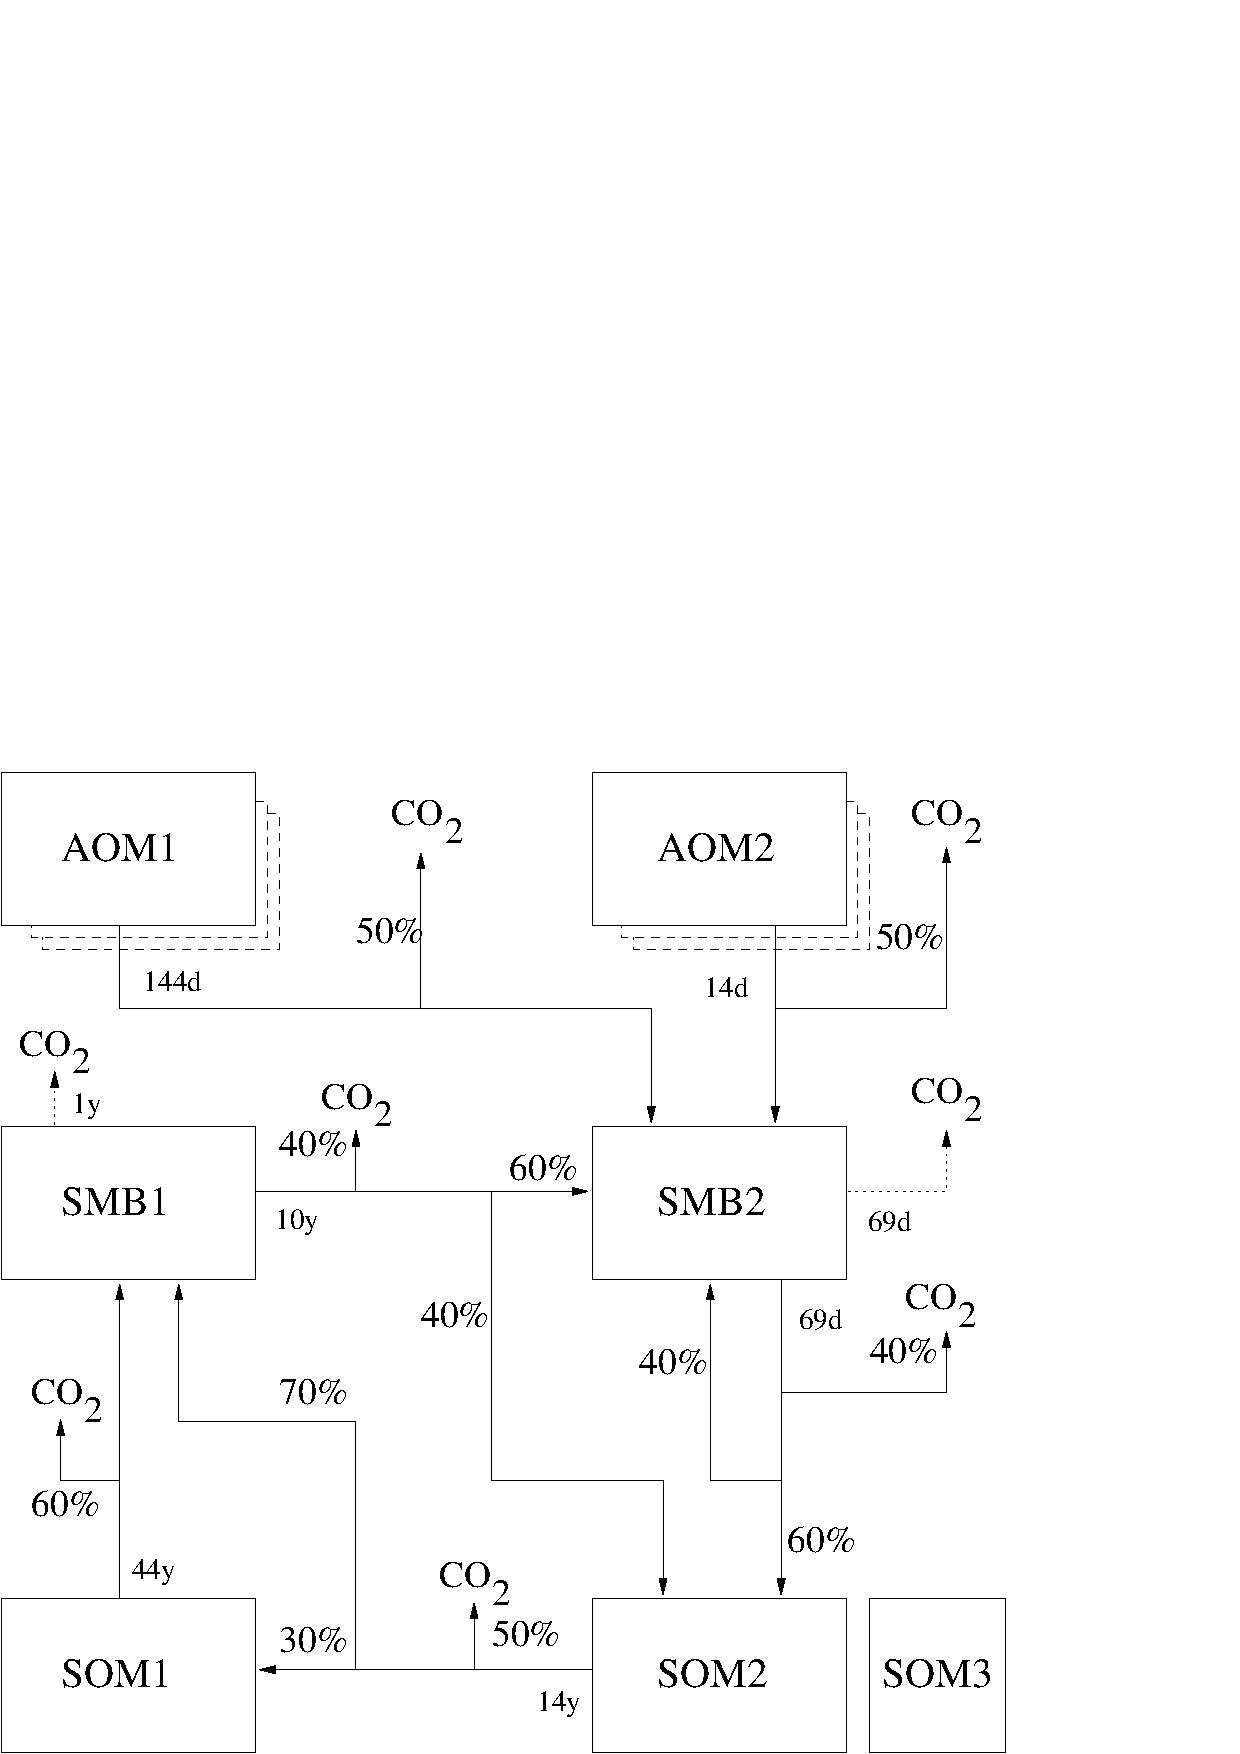
\includegraphics[width=0.8\hsize]{om2}

  \caption{Current standard organic matter model in \daisy{}.}
  \label{fig:om2}
\end{figure}

The amount of carbon turned over and decomposed is directly
proportional with the size of the pool. We call this the
\emph{turnover rate} by the soil microbial biomass. All the pools in
figure~\ref{fig:om2} have a fully drawn outgoing line. From the
\textsc{som1} pool the outgoing line is marked with the text
``44y''. This indicate the turnover rate of this particular pool and
the number is the corresponding halftime (i.e. 44 years for the
\textsc{som1} pool), which means that if there was no input to the
pool, the pool would be half the original size after 44 years. For
some pools this time is given in days, e.g.\ the \textsc{smb2} pool
has a turnover halftime of 69 days.

If we follow the line from \textsc{som1} it splits into two
parts. 60\% is completely mineralized and lost as CO$_2$, the rest is
allocated to the microbial biomass in the \textsc{smb1}
pool. Considering the \textsc{som2} pool, we see that 70\% of the
carbon not lost as CO$_2$, are allocated to the microbial biomass and
the remaining 30\% ends up in \textsc{som1}. Besides a turnover rate,
the two \textsc{smb} pools also have a maintenance rate. This rate
reflects the cost of staying alive, and is indicated by a stippled
line out of the \textsc{smb} pools. In general, the rates and even the
number of \textsc{aom} pools are variable, the rates given here are
just examples. Also, there can be many sets of added organic matter
pools, each set corresponds to a particular fertilizer or residual
with its specific parameters.

The coefficients of the turnover rate and maintenance of the pools is
affected by abiotic factors as clay content in the soil, soil
temperature and moisture. The halftimes listed in Figure~\ref{fig:om2}
corresponds to 0\% clay, 10$^\circ$C and field capacity (defined as 10
hPa). The halftimes will increase with increasing clay content,
decreasing temperature, or decreasing soil water content. Further
information of the abiotic factors included in the organic matter
model in \daisy{} is given in \citet{daisy-def}.

\subsection{Evolution of the \daisy{} user base}

The original development of \daisy{} was founded by the Danish
Environmental Protection Agency \citep{daisy-def}, and the first
non-research use was made by expert users who evaluated the national
environmental plans for limiting nitrogen contamination of groundwater
and surface water \citep{VMP}. Since then, \daisy{} has been used in
other parts of the environmental and agricultural agencies \citep{MST,
  novana} and increasingly by local authorities for evaluating
regional plans \citep{novanastor} and for evaluation of applications
for changed farm practice at an individual farm level
\citep{plantinfo-daisy}. For the last case, \daisy{} has also been
used by consulting agencies representing the farmers who wants to
change farming practice.

The effect of this increased use has been that the users is not only
"experts". Therefore, a project was started in order to provide
standardized procedures for \daisy{} simulations
\citep{daisy-staabi}. As part of this project, most components of
\daisy{} was evaluated in order to find parameters and submodels which
could be initialized automatically from default values, or from other
parameters. These parameters and submodels are still available to the
expert user, but are hidden for the user who do not have the expertise
or data available. The result is that the software now appears much
simpler to the user, even though no substantial changes to the model
have been made.

Initialization of the partition of the organic matter into the various
soil pools have been a particular stumbling block for most users,
partly because the partition does not reflect an easily identifiable
property of the system being modeled.  This lead to the development of
a subsystem for initialization of the organic matter pools based on a
static approximation of the dynamic model, which will be explored in
the next section.

\subsection{Initialization of the organic matter pools}

Daisy provides several mechanisms for initialization of the organic
matter pools, applicable in different situation.  The gratest amount
of control can be achieved by explicitly specifting the content of
each pool.  However, since this requires far more information of both
the soil and the model than the user can reasonably be expected to
possess, this initialization option is almost exclusively used in
connection with the ``hotstart'' facility, that is, restarting the
simulation from the saved state of an earlier simulation.

In order to simplify the initialization, a static approximation of the
dynamic organic matter turnover model is used.  The organic matter
model is dynamic due to the uneven application of \textsc{aom}, and
the weather dependent abiotic factors.  The static model is achieved
by considering average input of added organic matter, and effective
static values for the abiotic factors.  If we assume the dynamic model
is not strongly dependent of the initial conditions, we can combine
this initial estimate with a warmup period, to achive a reasonable
initial state for the period we are interested in simulating.

For typical use of \daisy{} (agricultural soil with annual or biannual
crops) this works well for the initialization of the \textsc{smb} and
\textsc{aom} pools.  After one or two years, the \textsc{smb} and
\textsc{aom} pools will have adjusted to level of input, and the
earlier history will be less relevant.  However, as shall be
demonstrated later, the \textsc{som} pools can take centuries to reach
equilibrium with new input levels.

The generalized form for dynamic change of the individual pools
($\Delta\mbox{\textsc{aom}}i$, $\Delta\mbox{\textsc{smb}}i$ and
$\Delta\mbox{\textsc{som}}j$) is shown in Equations~\ref{eq:dsmb},
\ref{eq:dsom} and \ref{eq:daom}:

\begin{equation}
   \begin{array}{rclcr}
      \label{eq:dsmb}
      \Delta\mbox{\textsc{smb}}i &=& \displaystyle
      \sum_{k=1}^{\mbox{\tiny\#\textsc{smb}}} a_{i,k}\,\mbox{\textsc{smb}}k +
      \sum_{l=1}^{\mbox{\tiny\#\textsc{som}}} b_{i,l}\,\mbox{\textsc{som}}l +
      \sum_{m=1}^{\mbox{\tiny\#\textsc{som}}} c_{i,m}\,\mbox{\textsc{aom}}m
      &;&i = 1\ldots\mbox{\#\textsc{smb}}
   \end{array}
\end{equation}
\begin{equation}
   \begin{array}{rclcr}
      \label{eq:dsom}
      \Delta\mbox{\textsc{som}}j &=& \displaystyle
      \sum_{k=1}^{\mbox{\tiny\#\textsc{smb}}} d_{j,k}\,\mbox{\textsc{smb}}k +
      \sum_{l=1}^{\mbox{\tiny\#\textsc{som}}} e_{j,l}\,\mbox{\textsc{som}}l +
      \sum_{m=1}^{\mbox{\tiny\#\textsc{som}}} f_{j,m}\,\mbox{\textsc{aom}}m
      &;&j = 1\ldots\mbox{\#\textsc{som}}
   \end{array}
\end{equation}

Static model
  General equations for smb, som, aom, & total
  Specific version for the simulation in the next chapter.

Solutions

  Knowns and unknowns, linear equations.

  Explicit som partitioning
  Equilibrium 
    (delta SMB & delta SOM = 0)
    SOM3, TOTAL, delta AOM ukendt
    1. SOM3 ukendt, subsoil
    2. TOTAL ukendt, next section
    3. delta AOM ukendt
  Quasi-equilibrium
    delta SOM1 ukendt
  C/N fixed, delta N kendt
  
Next: Compare Eq-3, Quasi-eq og lang opvarmning
\end{verbatim}

\subsection{Initializing the standard organic matter model}

The first step of a new initialization procedure was conducted by
\citet{daisy-init}. They found that the ratio between the \textsc{som1}
and \textsc{som2} for a system in equilibrium would be 49\% vs
51\%. This recalibration required the users to readjust the
partitioning between \textsc{som1} and \textsc{som2}. However, there
was a strong tendency that the "non-experts" users just picked the
equilibrium values.  As this was usually a poor


In \daisy{} the current standard to initialize the partition between
the organic pools is to use an equilibrium assumption. There are two
conditions where equilibrium is a good assumption: 1) when the system
quickly reach equilibrium compared to the external imposed changes, or
2) when the dynamic of the system quickly dominate over the initial
condition. The assumption of an initial equilibrium is good when a
reasonable initial state is needed rather than a correct one. However,
as depicted in the introduction the time to reach equilibrium in the
soil organic matter system is measured in centuries and the long term
simulations of organic matter dynamics are dependent on the initial
amount of \textsc{som2}.

The calibration of the current standard \daisy{} model is based
primarily on measurements on agricultural topsoil
\citep{daisy-somnew,mueller-smb}, where all the humus is presumed to
be active. This means the calibration is not suitable for subsoils,
nor for some humus-rich topsoils. The \textsc{som3} pool in
Figure~\ref{fig:om2} exists to compensate for these shortcomings. The
\textsc{som3} pool is inert and does not participate in the organic
matter turnover. The inert humus still affects other aspects of
\daisy{}, such as the hydraulic and adsorption properties of the
soil. For the subsoil, it is assumed that the system is in equilibrium
with the input, and park enough humus in the \textsc{som3} pool so
that this assumption holds true. The observant reader will remember
that we earlier argued that the equilibrium assumption is
wrong. However, by definition the organic matter in the subsoil
contributes relatively little to the total system so this assumption
is good enough. For the topsoil, the user can explicitly put some of
the humus in the \textsc{som3} pool, for instance for humus-rich
topsoils.

\section{Methodology}

Static model

Dynamic model

\subsection{Basic equations}

In order to find a better way to initialize the organic matter pools, we will start by looking at the four equations describing their internal relationships:
\begin{eqnarray}
  \Delta\mbox{\textsc{smb1}} &=& a\> \mbox{\textsc{smb1}} + b\>
  \mbox{\textsc{smb2}} + c\> \mbox{\textsc{som1}} + d\>
  \mbox{\textsc{som2}} + e\, \Delta\mbox{\textsc{aom}}\label{eq:dsmb1}\\
  \Delta\mbox{\textsc{smb2}} &=& f\> \mbox{\textsc{smb1}} + g\>
  \mbox{\textsc{smb2}} + h\> \mbox{\textsc{som1}} + i\>
  \mbox{\textsc{som2}} + j\, \Delta\mbox{\textsc{aom}}\label{eq:dsmb2}\\
  \Delta\mbox{\textsc{som1}} &=& k\> \mbox{\textsc{smb1}} + l\>
  \mbox{\textsc{smb2}} + m\> \mbox{\textsc{som1}} + n\>
  \mbox{\textsc{som2}} + o\, \Delta\mbox{\textsc{aom}}\\
  \Delta\mbox{\textsc{som2}} &=& p\> \mbox{\textsc{smb1}} + q\>
  \mbox{\textsc{smb2}} + r\> \mbox{\textsc{som1}} + s\>
  \mbox{\textsc{som2}} + t\, \Delta\mbox{\textsc{aom}}\label{eq:dsom2}
\end{eqnarray}
The change of matter in the organic pools ($\Delta\mbox{\textsc{smb1}}$, $\Delta\mbox{\textsc{smb2}}$, $\Delta\mbox{\textsc{som1}}$, $\Delta\mbox{\textsc{som2}}$) in Equation~(\ref{eq:dsmb1})-(\ref{eq:dsom2}) are described by the content (\textsc{smb1}, \textsc{smb2}, \textsc{som1}, or \textsc{som2}) and the factors $a$ to $t$. The \textsc{aom} pools are excluded in above equations as they do not receive any input from the other pools. They only receive input from outside sources such as crop residuals and fertilizer which can be ignored in the initialization procedure. However, the $\Delta\mbox{\textsc{aom}}$, are a source to the other pools and represents the total carbon input to the system.

The factors $a$ to $t$ depend on the model. Hence, the factors are different in the the recalibrated model (Figure~\ref{fig:om2}) from the original model (Figure~\ref{fig:om1}). They also depend on the the abiotic factors in the model as the clay content, the soil temperature and water potential. Some of the factors may be zero. For example, no carbon is allocated directly from the \textsc{aom} pools to the \textsc{som1} pool, so $o$ will be zero. For instance, to calculate $f$ from equation~(\ref{eq:dsmb2}) the following equation can be listed:
\begin{equation}
  \label{eq:f}
  f = (t_{\mbox{\tiny\textsc{smb1}}}\,
  (X_{\mbox{\tiny\textsc{smb1}}\rightarrow{\mbox{\tiny\textsc{smb2}}}}\,
  E_{\mbox{\tiny\textsc{smb1}}}
  - 1) - m_{\mbox{\tiny\textsc{smb1}}})\,
  F_{\mbox{\tiny\textsc{smb1}}}^T (T)\,
  F_{\mbox{\tiny\textsc{smb1}}}^\psi (\psi)\,
  F_{\mbox{\tiny\textsc{smb1}}}^C (X_c)
\end{equation}
where $t_{\mbox{\tiny\textsc{smb1}}}$ is the turnover rate and $m_{\mbox{\tiny\textsc{smb1}}}$ is the maintenance of the \textsc{smb1} pool. $X_{\mbox{\tiny\textsc{smb1}}\rightarrow{\mbox{\tiny\textsc{smb2}}}}$ is the carbon fraction going from \textsc{smb1} to \textsc{smb2}. $E_{\mbox{\tiny\textsc{smb1}}}$ is the efficiency of which \textsc{smb1} can be decomposed, the remaining part is lost to the atmosphere as CO$_2$. $F_{\mbox{\tiny\textsc{smb1}}}^T$, $F_{\mbox{\tiny\textsc{smb1}}}^\psi$, and $F_{\mbox{\tiny\textsc{smb1}}}^C$ are functions describing the effect of the  abiotic factors for soil temperature, moisture, and clay, respectively. The other factors in Equation~(\ref{eq:dsmb1})-(\ref{eq:dsom2}) can be described by similar forms. The factors are variables as soil temperature ($T$) as well as soil moisture ($\psi$) are variables and changes over time. The clay content is assumed to be constant and specified by the user.

To ensure a robust way of initialization, with regard to changes in the model, the factors $a$ to $t$ are included in the initialization procedure. If only two pools are defined, \textsc{som} and \textsc{smb}, there are four equations (Equation~(\ref{eq:dsmb1})-(\ref{eq:dsom2})) and nine unknowns ($\Delta\mbox{\textsc{smb1}}$, $\Delta\mbox{\textsc{smb2}}$, $\Delta\mbox{\textsc{som1}}$, $\Delta\mbox{\textsc{som2}}$, $\Delta\mbox{\textsc{aom}}$, \textsc{smb1}, \textsc{smb2}, \textsc{som1}, \textsc{som2}). To solve this, more information is needed. The total organic matter content in the field, can be directly measured. This information gives one new equation (Equation~(\ref{eq:total})) and two new variables (\textsc{total} and \textsc{aom}) where the initial content of \mbox{\textsc{aom}} may be given a default value corresponding to typical root residuals left on the field.
\begin{equation}
  \label{eq:total}
  \mbox{\textsc{total}} = \mbox{\textsc{smb1}} + \mbox{\textsc{smb2}}
  + \mbox{\textsc{som1}} + \mbox{\textsc{som2}} + \mbox{\textsc{aom}}
\end{equation}

By assuming quasi-equilibrium in the initialization procedure, the slowest pool (\textsc{som1}) is allowed to change. The physical interpretation of this initialization is that all except for the slowest pool have reached a quasi-equilibrium with respect to the input and the size of the slowest pool. When it is assumed that the slowest pool is still changing (and the other pools will have to change to reflect that), this is not a true equilibrium. Hence, in the quasi-equilibrium it is assumed:
\begin{eqnarray}
  \Delta\mbox{\textsc{smb1}} &=& 0\\
  \Delta\mbox{\textsc{smb2}} &=& 0\\
  \Delta\mbox{\textsc{som2}} &=& 0\label{eq:fastpooleq}\\
  \Delta\mbox{\textsc{aom}} &=& u\label{eq:daom}
\end{eqnarray}
This requires that the user specifies the carbon input ($u$) to the system. We now have nine equations (Equations (\ref{eq:dsmb1})-(\ref{eq:dsom2}) and (\ref{eq:total})-(\ref{eq:daom})) with six unknowns ($\Delta\mbox{\textsc{som1}}$, $\Delta\mbox{\textsc{aom}}$, \textsc{smb1}, \textsc{smb2}, \textsc{som1}, \textsc{som2}) to initialize the system which can be solved.

\subsection{Selected soils and management}
For evaluate the use of assuming quasi-equilibrium in initializing soil organic matter, long-term organic matter simulations have been conducted using Danish management as well as Danish climate and soils. Two standard soils for Danish conditions have been selected, a coarse sandy soil and a sandy loam soil. The particle size distribution of the two soils are listed in Table (\ref{tab:psd}).

\begin{table}[htbp]
  \caption{Particle size distribution of the two standard soils.}
  \label{tab:psd}
\vspace{0.25cm}
\begin{tabular}{c c c c}
  \hline
  Soil         &  clay  & silt    & sand \\
               & (<2 $�$m) & (2-50 $�$m) & (50-2000 $�$m)\\\hline
  Coarse sandy & 3.9    & 6.4     & 89.7\\
  Sandy loam   & 12.4   & 24.9    & 62.7\\\hline
\end{tabular}
\end{table}

Two management practice of high and low C-input to the simulated systems have been evaluated for each soil. For the coarse sandy soil also a medium C-input management was included. Table (\ref{tab:soils}) lists the average C-input  together with the average and initial abiotic factor and the initial C-input of the different management and soil combinations.

\begin{table}[htbp]
  \caption{Average input of organic C and average abiotic factor in simulated management for sandy and sandy loam soils. The initial abiotic factor and initial C refers to the initialization of the organic matter module using equilibrium assumptions.}
  \label{tab:soils}
\vspace{0.25cm}
\begin{tabular}{c c c c c}
  \hline
       &            & average & average (and initial)  & initial \\
  Soil & Management & C input & abiotic factor         & C input \\
       &            & (kg C ha$^{-1}$ y$^{-1}$)&       & (kg C ha$^{-1}$ y$^{-1}$)\\\hline
  Sandy & Low       & 1817 & 0.680 & 5200\\
  Sandy & Medium    & 4412 & 0.680 & 5200\\
  Sandy & High      & 5158 & 0.681 & 1800\\
  Sandy loam & Low  & 2283 & 0.622 & 6500\\
  Sandy loam & High & 6525 & 0.623 & 2300\\\hline
\end{tabular}
\end{table}

\subsection{Initialization of abiotic factors}
For the initialization we must use constant values. By default the Daisy model use the local average air temperature (which is already specified by the user in the weather file) for $T$, and field capacity (10 hPa) for $\psi$. Since the function $F^T$ is non-linear, using the average is incorrect. In particular, $F^T$ is zero for $T < 0^\circ$C, so for a cold climate like the Danish the significance of frost is overestimated. On the other hand, using pF 2 may be acceptable for the wet climate like in Denmark, but may be unreasonable for a dry climate. The two factors interact, so a low value for $F^T (T)$ is most significant when $F^\psi (\psi)$ is high, and vice-versa. By logging the product of factors in a realistic simulation, \daisy{} can be used to calculate the combined effect. From that, the user can choose values for $T$ and $\psi$ that give the same effect.

\section{Results and Discussion}

\subsection{Long term simulations}
 Figure~\ref{fig:JB6} shows humus content for a system that goes from equilibrium at a high level of carbon input, to equilibrium at a low level of carbon input. Figure~\ref{fig:JB6} also shows the simulated \textsc{som1} fraction of total \textsc{som}.

\begin{figure}[htbp]
% GNUPLOT: LaTeX picture with Postscript
\begingroup
  \makeatletter
  \providecommand\color[2][]{%
    \GenericError{(gnuplot) \space\space\space\@spaces}{%
      Package color not loaded in conjunction with
      terminal option `colourtext'%
    }{See the gnuplot documentation for explanation.%
    }{Either use 'blacktext' in gnuplot or load the package
      color.sty in LaTeX.}%
    \renewcommand\color[2][]{}%
  }%
  \providecommand\includegraphics[2][]{%
    \GenericError{(gnuplot) \space\space\space\@spaces}{%
      Package graphicx or graphics not loaded%
    }{See the gnuplot documentation for explanation.%
    }{The gnuplot epslatex terminal needs graphicx.sty or graphics.sty.}%
    \renewcommand\includegraphics[2][]{}%
  }%
  \providecommand\rotatebox[2]{#2}%
  \@ifundefined{ifGPcolor}{%
    \newif\ifGPcolor
    \GPcolortrue
  }{}%
  \@ifundefined{ifGPblacktext}{%
    \newif\ifGPblacktext
    \GPblacktexttrue
  }{}%
  % define a \g@addto@macro without @ in the name:
  \let\gplgaddtomacro\g@addto@macro
  % define empty templates for all commands taking text:
  \gdef\gplbacktext{}%
  \gdef\gplfronttext{}%
  \makeatother
  \ifGPblacktext
    % no textcolor at all
    \def\colorrgb#1{}%
    \def\colorgray#1{}%
  \else
    % gray or color?
    \ifGPcolor
      \def\colorrgb#1{\color[rgb]{#1}}%
      \def\colorgray#1{\color[gray]{#1}}%
      \expandafter\def\csname LTw\endcsname{\color{white}}%
      \expandafter\def\csname LTb\endcsname{\color{black}}%
      \expandafter\def\csname LTa\endcsname{\color{black}}%
      \expandafter\def\csname LT0\endcsname{\color[rgb]{1,0,0}}%
      \expandafter\def\csname LT1\endcsname{\color[rgb]{0,1,0}}%
      \expandafter\def\csname LT2\endcsname{\color[rgb]{0,0,1}}%
      \expandafter\def\csname LT3\endcsname{\color[rgb]{1,0,1}}%
      \expandafter\def\csname LT4\endcsname{\color[rgb]{0,1,1}}%
      \expandafter\def\csname LT5\endcsname{\color[rgb]{1,1,0}}%
      \expandafter\def\csname LT6\endcsname{\color[rgb]{0,0,0}}%
      \expandafter\def\csname LT7\endcsname{\color[rgb]{1,0.3,0}}%
      \expandafter\def\csname LT8\endcsname{\color[rgb]{0.5,0.5,0.5}}%
    \else
      % gray
      \def\colorrgb#1{\color{black}}%
      \def\colorgray#1{\color[gray]{#1}}%
      \expandafter\def\csname LTw\endcsname{\color{white}}%
      \expandafter\def\csname LTb\endcsname{\color{black}}%
      \expandafter\def\csname LTa\endcsname{\color{black}}%
      \expandafter\def\csname LT0\endcsname{\color{black}}%
      \expandafter\def\csname LT1\endcsname{\color{black}}%
      \expandafter\def\csname LT2\endcsname{\color{black}}%
      \expandafter\def\csname LT3\endcsname{\color{black}}%
      \expandafter\def\csname LT4\endcsname{\color{black}}%
      \expandafter\def\csname LT5\endcsname{\color{black}}%
      \expandafter\def\csname LT6\endcsname{\color{black}}%
      \expandafter\def\csname LT7\endcsname{\color{black}}%
      \expandafter\def\csname LT8\endcsname{\color{black}}%
    \fi
  \fi
  \setlength{\unitlength}{0.0500bp}%
  \begin{picture}(6120.00,3024.00)%
    \gplgaddtomacro\gplbacktext{%
      \csname LTb\endcsname%
      \put(1034,704){\makebox(0,0)[r]{\strut{} 0}}%
      \put(1034,1047){\makebox(0,0)[r]{\strut{} 0.2}}%
      \put(1034,1389){\makebox(0,0)[r]{\strut{} 0.4}}%
      \put(1034,1732){\makebox(0,0)[r]{\strut{} 0.6}}%
      \put(1034,2075){\makebox(0,0)[r]{\strut{} 0.8}}%
      \put(1034,2417){\makebox(0,0)[r]{\strut{} 1}}%
      \put(1034,2760){\makebox(0,0)[r]{\strut{} 1.2}}%
      \put(1166,484){\makebox(0,0){\strut{}2000}}%
      \put(1841,484){\makebox(0,0){\strut{}2100}}%
      \put(2517,484){\makebox(0,0){\strut{}2200}}%
      \put(3192,484){\makebox(0,0){\strut{}2300}}%
      \put(3867,484){\makebox(0,0){\strut{}2400}}%
      \put(4543,484){\makebox(0,0){\strut{}2500}}%
      \put(5218,484){\makebox(0,0){\strut{}2600}}%
      \put(5350,704){\makebox(0,0)[l]{\strut{} 20}}%
      \put(5350,1047){\makebox(0,0)[l]{\strut{} 30}}%
      \put(5350,1389){\makebox(0,0)[l]{\strut{} 40}}%
      \put(5350,1732){\makebox(0,0)[l]{\strut{} 50}}%
      \put(5350,2075){\makebox(0,0)[l]{\strut{} 60}}%
      \put(5350,2417){\makebox(0,0)[l]{\strut{} 70}}%
      \put(5350,2760){\makebox(0,0)[l]{\strut{} 80}}%
      \put(3192,154){\makebox(0,0){\strut{}Year}}%
    }%
    \gplgaddtomacro\gplfronttext{%
    }%
    \gplbacktext
    \put(0,0){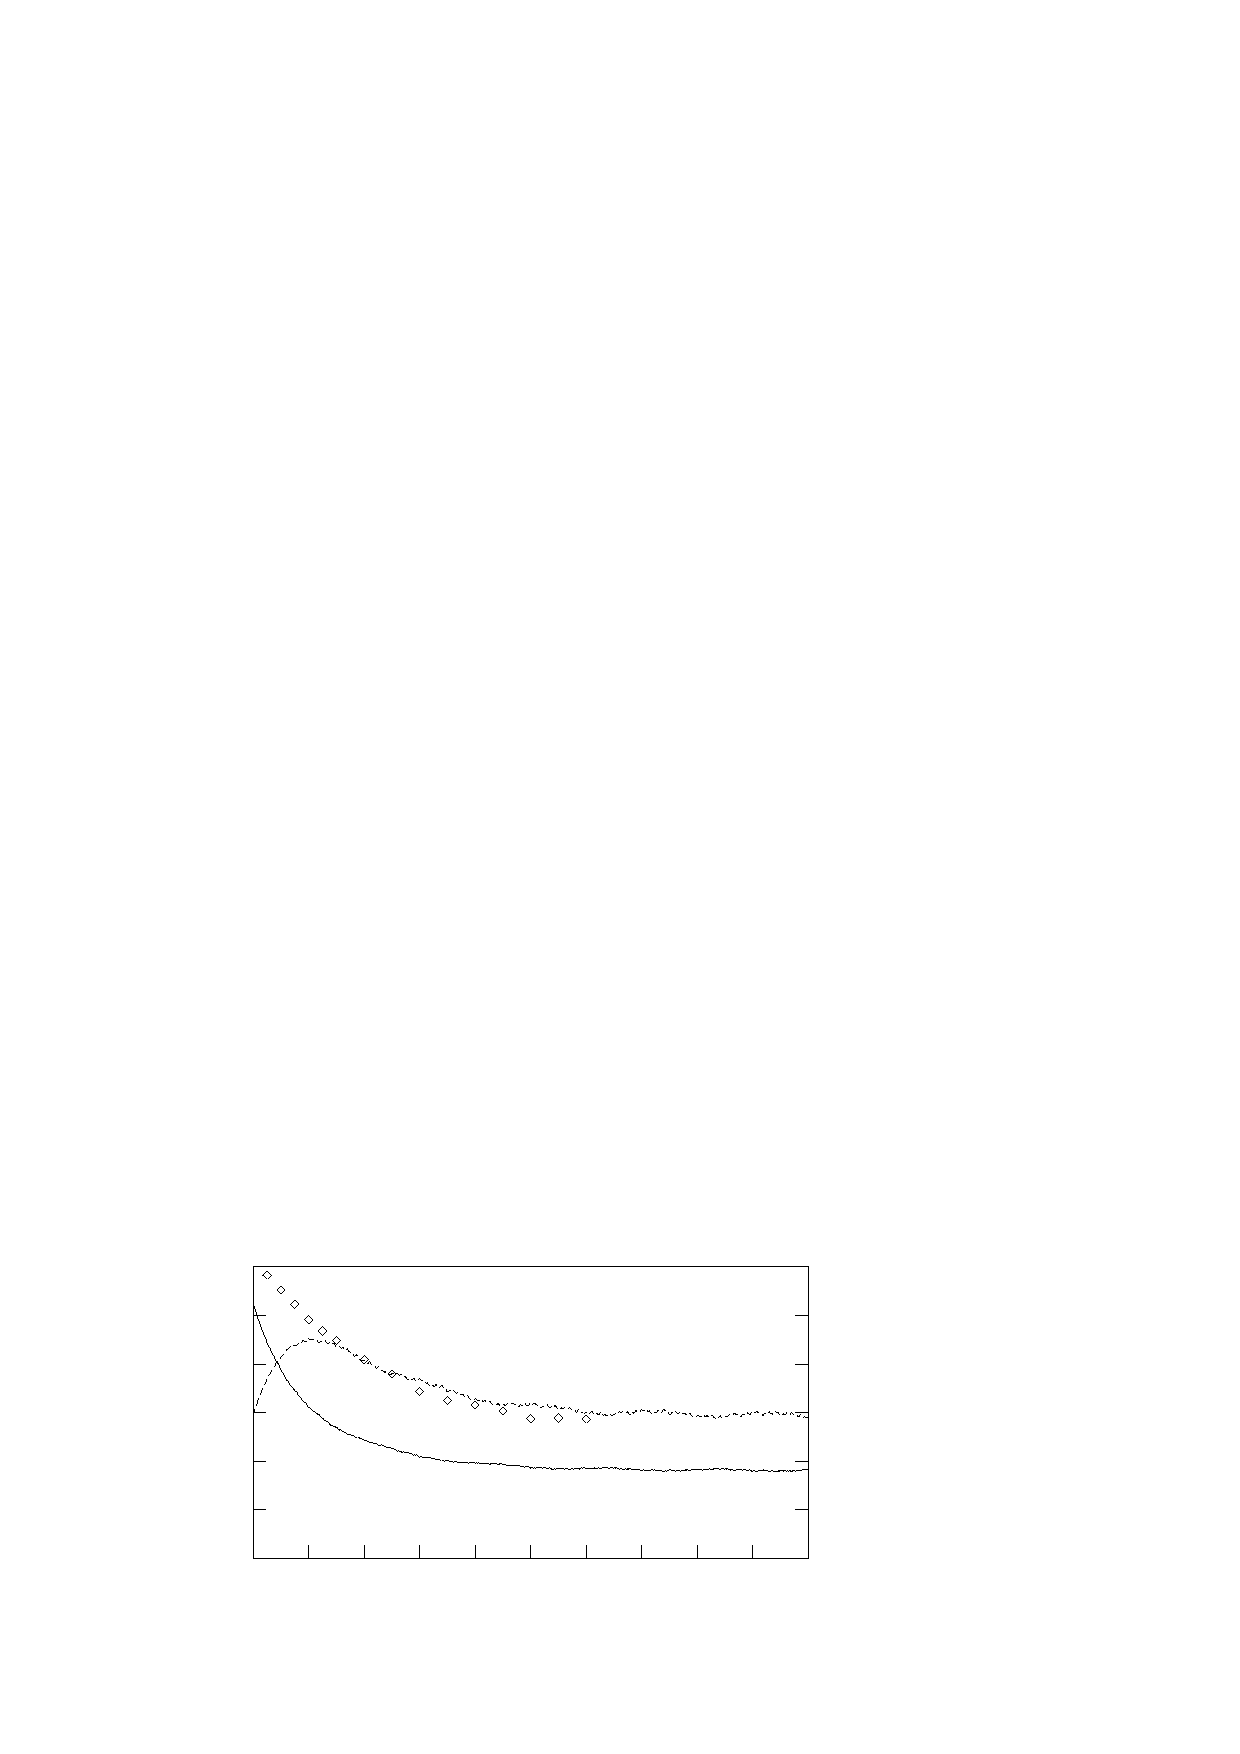
\includegraphics{realminJB6}}%
    \gplfronttext
  \end{picture}%
\endgroup

% GNUPLOT: LaTeX picture with Postscript
\begingroup
  \makeatletter
  \providecommand\color[2][]{%
    \GenericError{(gnuplot) \space\space\space\@spaces}{%
      Package color not loaded in conjunction with
      terminal option `colourtext'%
    }{See the gnuplot documentation for explanation.%
    }{Either use 'blacktext' in gnuplot or load the package
      color.sty in LaTeX.}%
    \renewcommand\color[2][]{}%
  }%
  \providecommand\includegraphics[2][]{%
    \GenericError{(gnuplot) \space\space\space\@spaces}{%
      Package graphicx or graphics not loaded%
    }{See the gnuplot documentation for explanation.%
    }{The gnuplot epslatex terminal needs graphicx.sty or graphics.sty.}%
    \renewcommand\includegraphics[2][]{}%
  }%
  \providecommand\rotatebox[2]{#2}%
  \@ifundefined{ifGPcolor}{%
    \newif\ifGPcolor
    \GPcolorfalse
  }{}%
  \@ifundefined{ifGPblacktext}{%
    \newif\ifGPblacktext
    \GPblacktexttrue
  }{}%
  % define a \g@addto@macro without @ in the name:
  \let\gplgaddtomacro\g@addto@macro
  % define empty templates for all commands taking text:
  \gdef\gplbacktext{}%
  \gdef\gplfronttext{}%
  \makeatother
  \ifGPblacktext
    % no textcolor at all
    \def\colorrgb#1{}%
    \def\colorgray#1{}%
  \else
    % gray or color?
    \ifGPcolor
      \def\colorrgb#1{\color[rgb]{#1}}%
      \def\colorgray#1{\color[gray]{#1}}%
      \expandafter\def\csname LTw\endcsname{\color{white}}%
      \expandafter\def\csname LTb\endcsname{\color{black}}%
      \expandafter\def\csname LTa\endcsname{\color{black}}%
      \expandafter\def\csname LT0\endcsname{\color[rgb]{1,0,0}}%
      \expandafter\def\csname LT1\endcsname{\color[rgb]{0,1,0}}%
      \expandafter\def\csname LT2\endcsname{\color[rgb]{0,0,1}}%
      \expandafter\def\csname LT3\endcsname{\color[rgb]{1,0,1}}%
      \expandafter\def\csname LT4\endcsname{\color[rgb]{0,1,1}}%
      \expandafter\def\csname LT5\endcsname{\color[rgb]{1,1,0}}%
      \expandafter\def\csname LT6\endcsname{\color[rgb]{0,0,0}}%
      \expandafter\def\csname LT7\endcsname{\color[rgb]{1,0.3,0}}%
      \expandafter\def\csname LT8\endcsname{\color[rgb]{0.5,0.5,0.5}}%
    \else
      % gray
      \def\colorrgb#1{\color{black}}%
      \def\colorgray#1{\color[gray]{#1}}%
      \expandafter\def\csname LTw\endcsname{\color{white}}%
      \expandafter\def\csname LTb\endcsname{\color{black}}%
      \expandafter\def\csname LTa\endcsname{\color{black}}%
      \expandafter\def\csname LT0\endcsname{\color{black}}%
      \expandafter\def\csname LT1\endcsname{\color{black}}%
      \expandafter\def\csname LT2\endcsname{\color{black}}%
      \expandafter\def\csname LT3\endcsname{\color{black}}%
      \expandafter\def\csname LT4\endcsname{\color{black}}%
      \expandafter\def\csname LT5\endcsname{\color{black}}%
      \expandafter\def\csname LT6\endcsname{\color{black}}%
      \expandafter\def\csname LT7\endcsname{\color{black}}%
      \expandafter\def\csname LT8\endcsname{\color{black}}%
    \fi
  \fi
  \setlength{\unitlength}{0.0500bp}%
  \begin{picture}(6120.00,3024.00)%
    \gplgaddtomacro\gplbacktext{%
      \csname LTb\endcsname%
      \put(1034,440){\makebox(0,0)[r]{\strut{} 0}}%
      \put(1034,827){\makebox(0,0)[r]{\strut{} 0.2}}%
      \put(1034,1213){\makebox(0,0)[r]{\strut{} 0.4}}%
      \put(1034,1600){\makebox(0,0)[r]{\strut{} 0.6}}%
      \put(1034,1987){\makebox(0,0)[r]{\strut{} 0.8}}%
      \put(1034,2373){\makebox(0,0)[r]{\strut{} 1}}%
      \put(1034,2760){\makebox(0,0)[r]{\strut{} 1.2}}%
      \put(1166,220){\makebox(0,0){\strut{}2000}}%
      \put(1841,220){\makebox(0,0){\strut{}2100}}%
      \put(2517,220){\makebox(0,0){\strut{}2200}}%
      \put(3192,220){\makebox(0,0){\strut{}2300}}%
      \put(3867,220){\makebox(0,0){\strut{}2400}}%
      \put(4543,220){\makebox(0,0){\strut{}2500}}%
      \put(5218,220){\makebox(0,0){\strut{}2600}}%
      \put(5350,440){\makebox(0,0)[l]{\strut{} 20}}%
      \put(5350,827){\makebox(0,0)[l]{\strut{} 30}}%
      \put(5350,1213){\makebox(0,0)[l]{\strut{} 40}}%
      \put(5350,1600){\makebox(0,0)[l]{\strut{} 50}}%
      \put(5350,1987){\makebox(0,0)[l]{\strut{} 60}}%
      \put(5350,2373){\makebox(0,0)[l]{\strut{} 70}}%
      \put(5350,2760){\makebox(0,0)[l]{\strut{} 80}}%
    }%
    \gplgaddtomacro\gplfronttext{%
    }%
    \gplbacktext
    \put(0,0){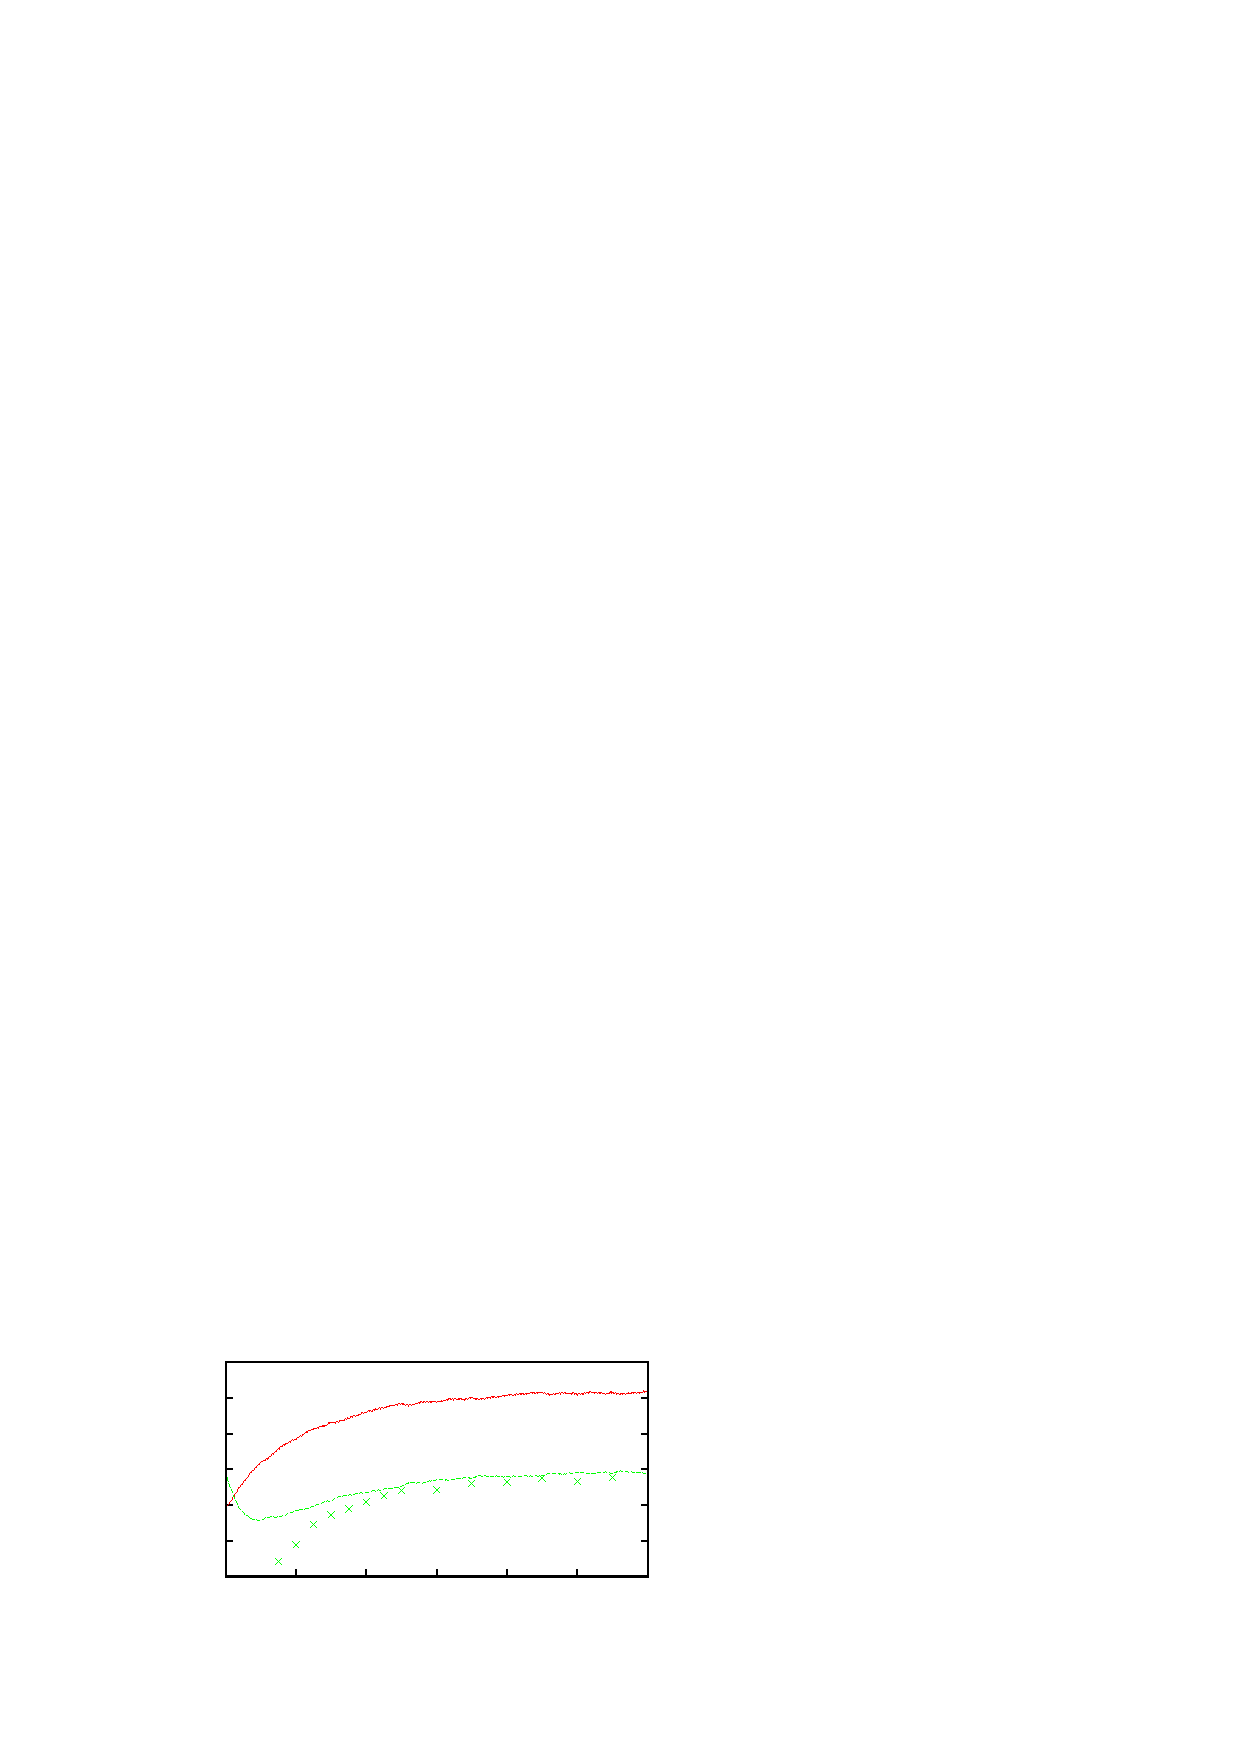
\includegraphics{realorgJB6}}%
    \gplfronttext
  \end{picture}%
\endgroup

 \caption{Long term simulation on a sandy loam soil of organic matter content (left axes)
    and \textsc{som1} fraction (right axes) with management changing from: (top) high to low C input and (bottom)low to    high C input. Simulated values are on the dotted line. The $\Diamond$'s indicate the initialization of \textsc{som1} for the current humus level estimated by the proposed quasi-equilibrium.}
  \label{fig:JB6}
\end{figure}

Figure~\ref{fig:JB1} shows that a simulation on a COARSE SANDY SOIL going from a low to high input equilibrium.

\begin{figure}[htbp]
%GNUPLOT: LaTeX picture with Postscript
\begin{picture}(0,0)%
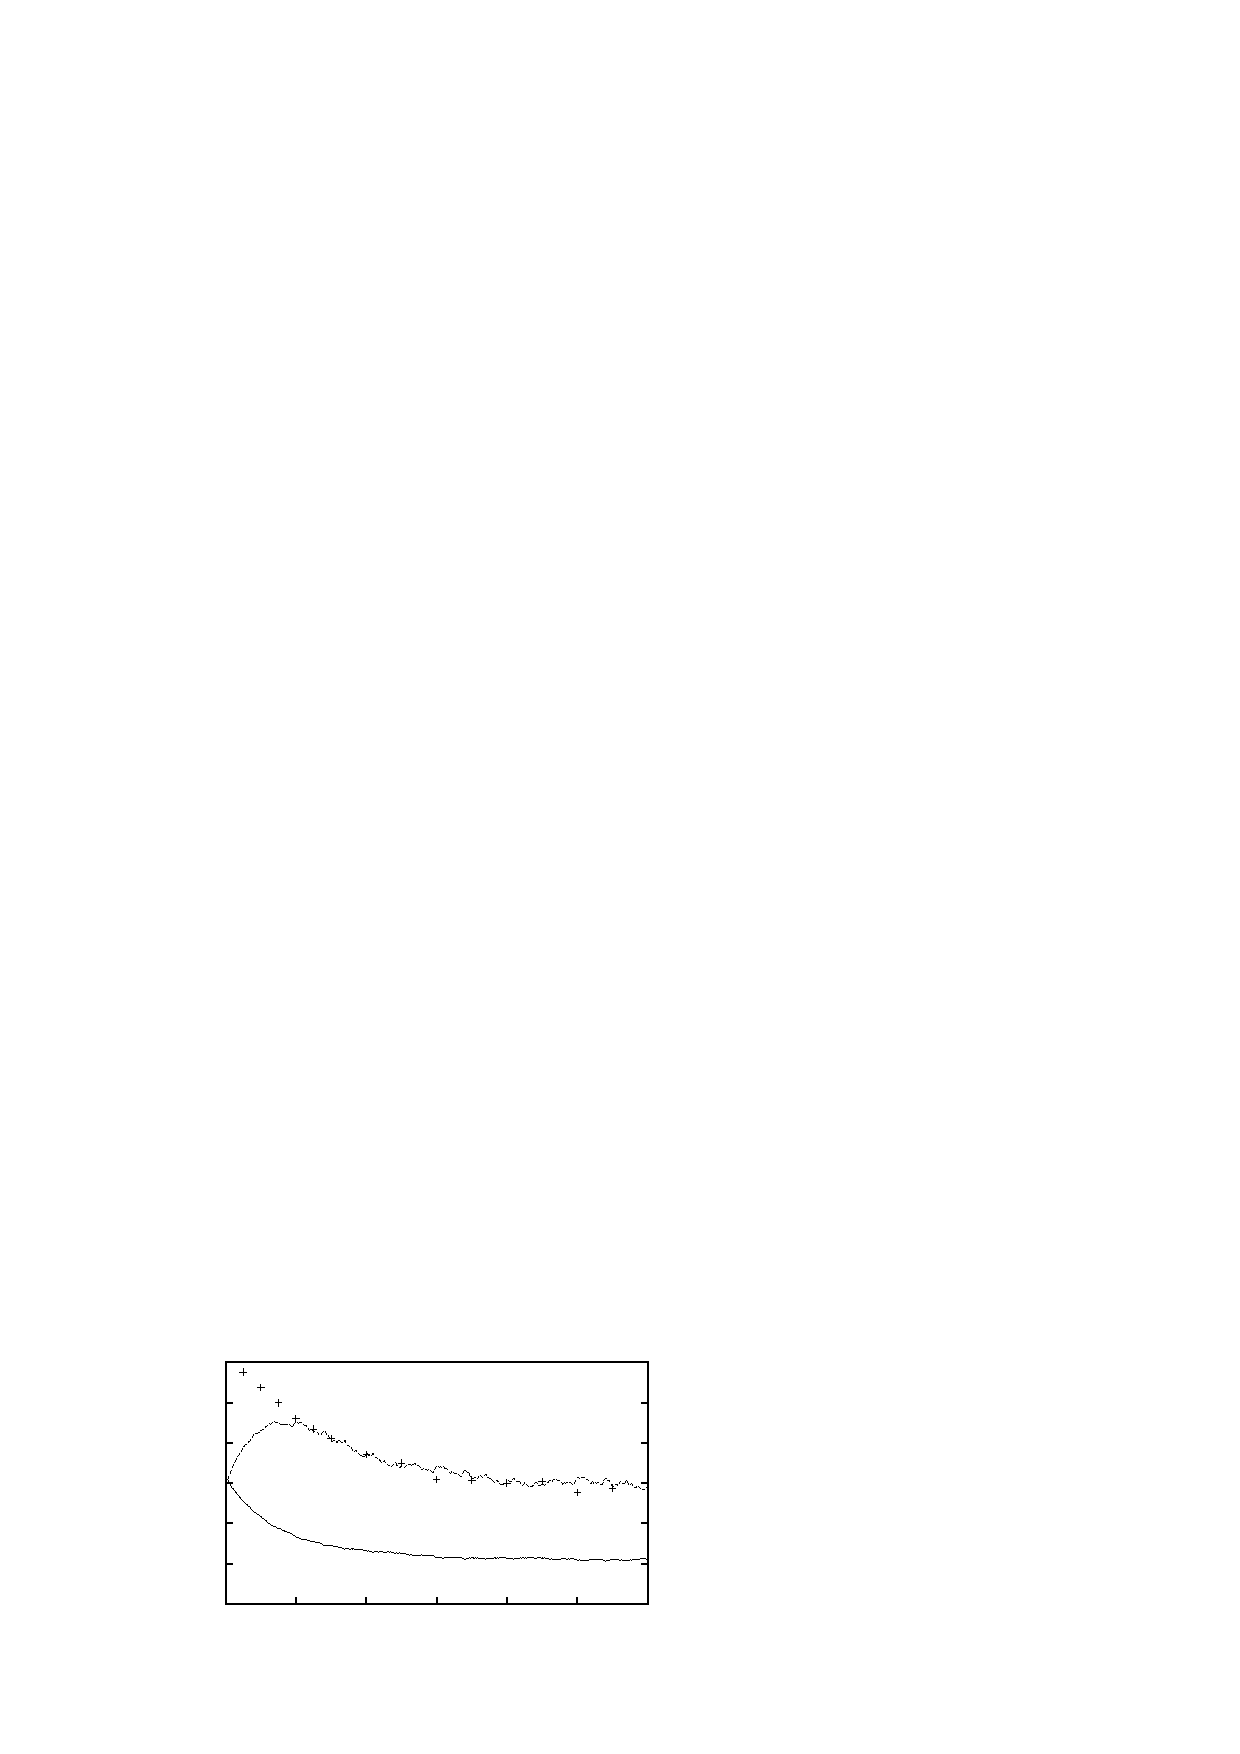
\includegraphics{realminJB1}%
\end{picture}%
\begingroup
\setlength{\unitlength}{0.0200bp}%
\begin{picture}(18000,8640)(0,0)%
\put(2200,1100){\makebox(0,0)[r]{\strut{} 0}}%
\put(2200,2265){\makebox(0,0)[r]{\strut{} 0.2}}%
\put(2200,3430){\makebox(0,0)[r]{\strut{} 0.4}}%
\put(2200,4595){\makebox(0,0)[r]{\strut{} 0.6}}%
\put(2200,5760){\makebox(0,0)[r]{\strut{} 0.8}}%
\put(2200,6925){\makebox(0,0)[r]{\strut{} 1}}%
\put(2200,8090){\makebox(0,0)[r]{\strut{} 1.2}}%
\put(2475,550){\makebox(0,0){\strut{}2000}}%
\put(3808,550){\makebox(0,0){\strut{}2100}}%
\put(5140,550){\makebox(0,0){\strut{}2200}}%
\put(6473,550){\makebox(0,0){\strut{}2300}}%
\put(7805,550){\makebox(0,0){\strut{}2400}}%
\put(9138,550){\makebox(0,0){\strut{}2500}}%
\put(10470,550){\makebox(0,0){\strut{}2600}}%
\put(11803,550){\makebox(0,0){\strut{}2700}}%
\put(13135,550){\makebox(0,0){\strut{}2800}}%
\put(14468,550){\makebox(0,0){\strut{}2900}}%
\put(15800,550){\makebox(0,0){\strut{}3000}}%
\put(16075,1100){\makebox(0,0)[l]{\strut{} 20}}%
\put(16075,2265){\makebox(0,0)[l]{\strut{} 30}}%
\put(16075,3430){\makebox(0,0)[l]{\strut{} 40}}%
\put(16075,4595){\makebox(0,0)[l]{\strut{} 50}}%
\put(16075,5760){\makebox(0,0)[l]{\strut{} 60}}%
\put(16075,6925){\makebox(0,0)[l]{\strut{} 70}}%
\put(16075,8090){\makebox(0,0)[l]{\strut{} 80}}%
\put(550,4595){\rotatebox{90}{\makebox(0,0){\strut{}Humus (\%)}}}%
\put(17449,4595){\rotatebox{90}{\makebox(0,0){\strut{}SOM1 (\%)}}}%
\end{picture}%
\endgroup
\endinput

%GNUPLOT: LaTeX picture with Postscript
\begin{picture}(0,0)%
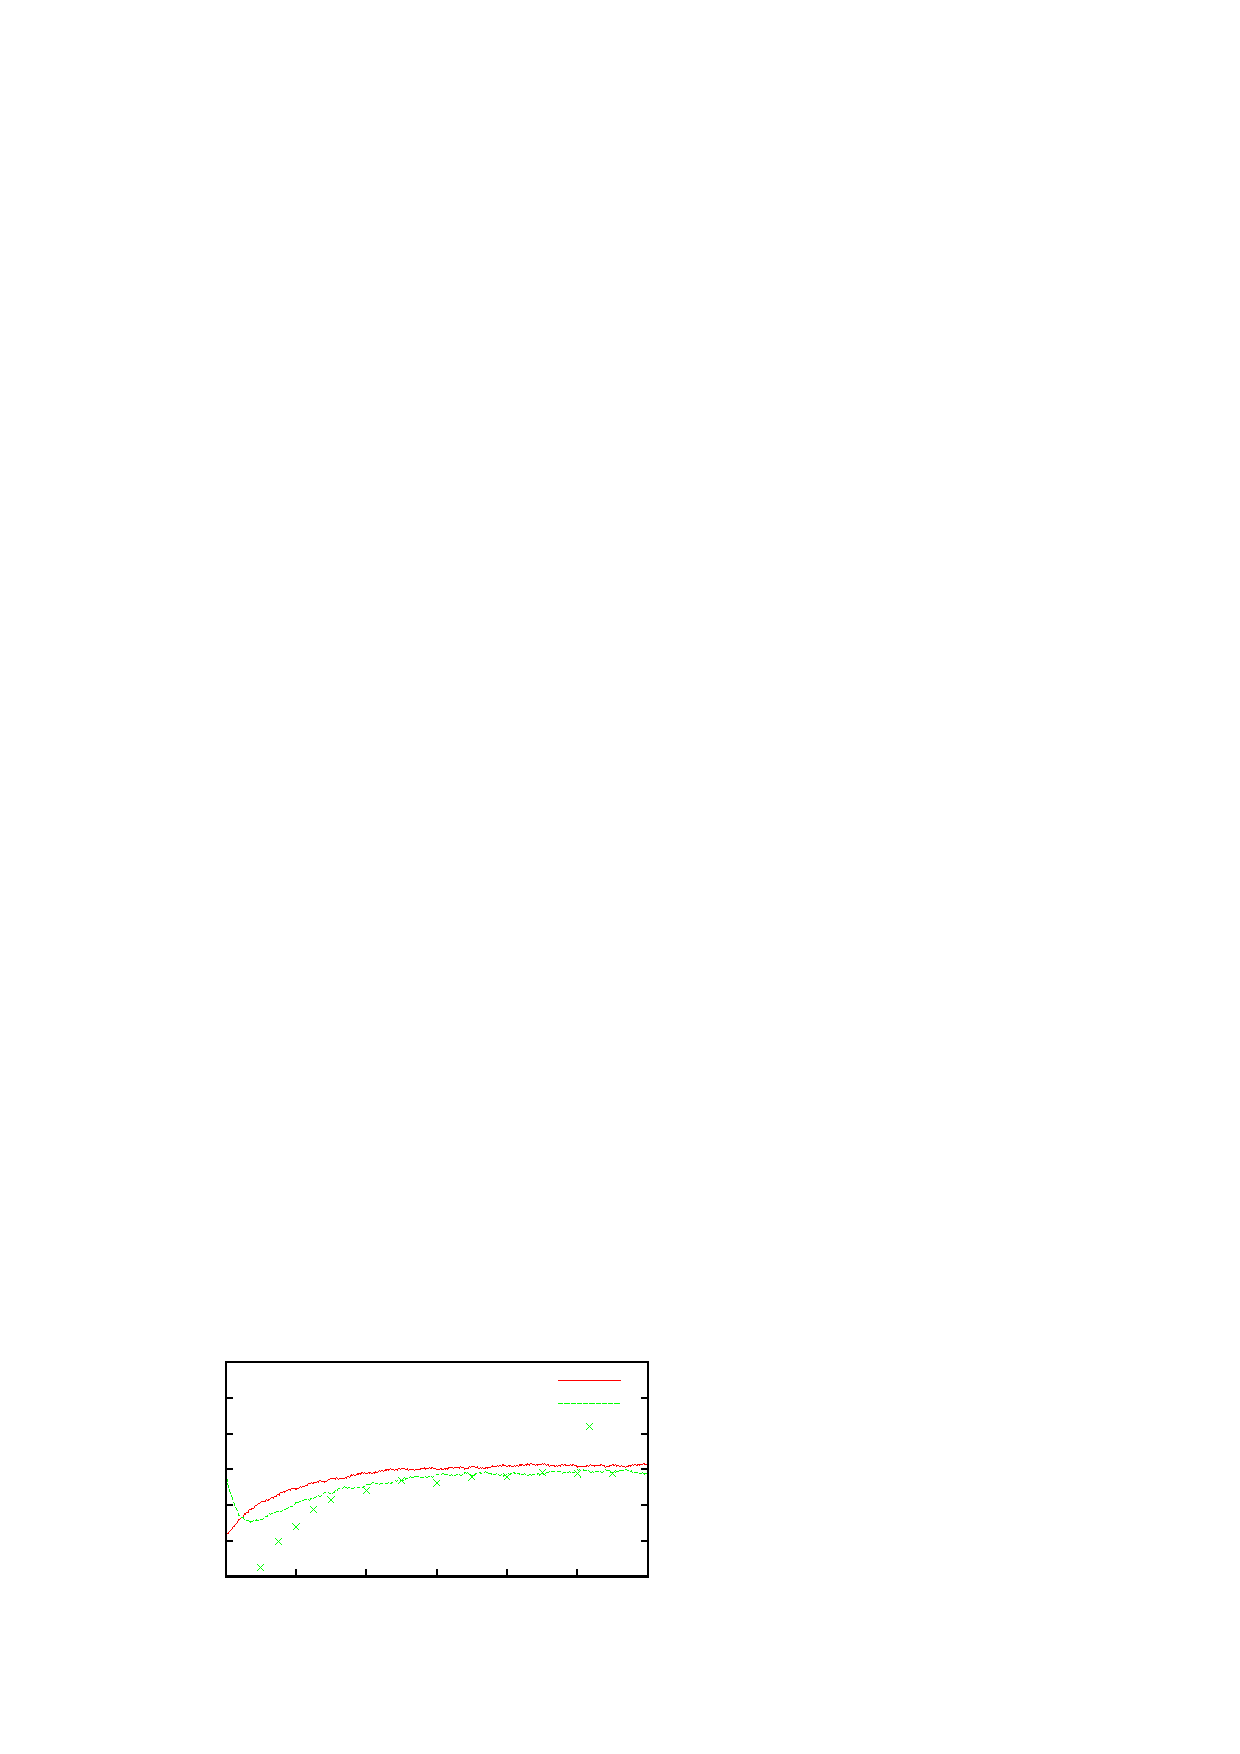
\includegraphics{realorgJB1}%
\end{picture}%
\begingroup
\setlength{\unitlength}{0.0200bp}%
\begin{picture}(18000,10800)(0,0)%
\put(2200,3300){\makebox(0,0)[r]{\strut{} 0}}%
\put(2200,4458){\makebox(0,0)[r]{\strut{} 0.2}}%
\put(2200,5617){\makebox(0,0)[r]{\strut{} 0.4}}%
\put(2200,6775){\makebox(0,0)[r]{\strut{} 0.6}}%
\put(2200,7933){\makebox(0,0)[r]{\strut{} 0.8}}%
\put(2200,9092){\makebox(0,0)[r]{\strut{} 1}}%
\put(2200,10250){\makebox(0,0)[r]{\strut{} 1.2}}%
\put(2475,2750){\makebox(0,0){\strut{}2000}}%
\put(3808,2750){\makebox(0,0){\strut{}2100}}%
\put(5140,2750){\makebox(0,0){\strut{}2200}}%
\put(6473,2750){\makebox(0,0){\strut{}2300}}%
\put(7805,2750){\makebox(0,0){\strut{}2400}}%
\put(9138,2750){\makebox(0,0){\strut{}2500}}%
\put(10470,2750){\makebox(0,0){\strut{}2600}}%
\put(11803,2750){\makebox(0,0){\strut{}2700}}%
\put(13135,2750){\makebox(0,0){\strut{}2800}}%
\put(14468,2750){\makebox(0,0){\strut{}2900}}%
\put(15800,2750){\makebox(0,0){\strut{}3000}}%
\put(16075,3300){\makebox(0,0)[l]{\strut{} 20}}%
\put(16075,4458){\makebox(0,0)[l]{\strut{} 30}}%
\put(16075,5617){\makebox(0,0)[l]{\strut{} 40}}%
\put(16075,6775){\makebox(0,0)[l]{\strut{} 50}}%
\put(16075,7933){\makebox(0,0)[l]{\strut{} 60}}%
\put(16075,9092){\makebox(0,0)[l]{\strut{} 70}}%
\put(16075,10250){\makebox(0,0)[l]{\strut{} 80}}%
\put(550,6775){\rotatebox{90}{\makebox(0,0){\strut{}Humus (\%)}}}%
\put(17449,6775){\rotatebox{90}{\makebox(0,0){\strut{}SOM1 (\%)}}}%
\put(9137,1925){\makebox(0,0){\strut{}Year}}%
\put(3687,825){\makebox(0,0)[l]{\strut{}Humus}}%
\put(3687,275){\makebox(0,0)[l]{\strut{}SOM1}}%
\put(12137,825){\makebox(0,0)[l]{\strut{}SOM1 quasi-equilibrium}}%
\end{picture}%
\endgroup
\endinput

  \caption{Long term simulation on a sandy soil of organic matter content (left axis)
    and \textsc{som1} fraction (right axis) with management changing from: (top) high to low C input and (bottom)low to    high C input. Simulated values are on the dotted line. The $\Diamond$'s indicate the initialization of \textsc{som1} for the current humus level estimated by the proposed quasi-equilibrium.}
  \label{fig:JB1}
\end{figure}

\begin{figure}[htbp]
% GNUPLOT: LaTeX picture with Postscript
\begingroup
  \makeatletter
  \providecommand\color[2][]{%
    \GenericError{(gnuplot) \space\space\space\@spaces}{%
      Package color not loaded in conjunction with
      terminal option `colourtext'%
    }{See the gnuplot documentation for explanation.%
    }{Either use 'blacktext' in gnuplot or load the package
      color.sty in LaTeX.}%
    \renewcommand\color[2][]{}%
  }%
  \providecommand\includegraphics[2][]{%
    \GenericError{(gnuplot) \space\space\space\@spaces}{%
      Package graphicx or graphics not loaded%
    }{See the gnuplot documentation for explanation.%
    }{The gnuplot epslatex terminal needs graphicx.sty or graphics.sty.}%
    \renewcommand\includegraphics[2][]{}%
  }%
  \providecommand\rotatebox[2]{#2}%
  \@ifundefined{ifGPcolor}{%
    \newif\ifGPcolor
    \GPcolorfalse
  }{}%
  \@ifundefined{ifGPblacktext}{%
    \newif\ifGPblacktext
    \GPblacktexttrue
  }{}%
  % define a \g@addto@macro without @ in the name:
  \let\gplgaddtomacro\g@addto@macro
  % define empty templates for all commands taking text:
  \gdef\gplbacktext{}%
  \gdef\gplfronttext{}%
  \makeatother
  \ifGPblacktext
    % no textcolor at all
    \def\colorrgb#1{}%
    \def\colorgray#1{}%
  \else
    % gray or color?
    \ifGPcolor
      \def\colorrgb#1{\color[rgb]{#1}}%
      \def\colorgray#1{\color[gray]{#1}}%
      \expandafter\def\csname LTw\endcsname{\color{white}}%
      \expandafter\def\csname LTb\endcsname{\color{black}}%
      \expandafter\def\csname LTa\endcsname{\color{black}}%
      \expandafter\def\csname LT0\endcsname{\color[rgb]{1,0,0}}%
      \expandafter\def\csname LT1\endcsname{\color[rgb]{0,1,0}}%
      \expandafter\def\csname LT2\endcsname{\color[rgb]{0,0,1}}%
      \expandafter\def\csname LT3\endcsname{\color[rgb]{1,0,1}}%
      \expandafter\def\csname LT4\endcsname{\color[rgb]{0,1,1}}%
      \expandafter\def\csname LT5\endcsname{\color[rgb]{1,1,0}}%
      \expandafter\def\csname LT6\endcsname{\color[rgb]{0,0,0}}%
      \expandafter\def\csname LT7\endcsname{\color[rgb]{1,0.3,0}}%
      \expandafter\def\csname LT8\endcsname{\color[rgb]{0.5,0.5,0.5}}%
    \else
      % gray
      \def\colorrgb#1{\color{black}}%
      \def\colorgray#1{\color[gray]{#1}}%
      \expandafter\def\csname LTw\endcsname{\color{white}}%
      \expandafter\def\csname LTb\endcsname{\color{black}}%
      \expandafter\def\csname LTa\endcsname{\color{black}}%
      \expandafter\def\csname LT0\endcsname{\color{black}}%
      \expandafter\def\csname LT1\endcsname{\color{black}}%
      \expandafter\def\csname LT2\endcsname{\color{black}}%
      \expandafter\def\csname LT3\endcsname{\color{black}}%
      \expandafter\def\csname LT4\endcsname{\color{black}}%
      \expandafter\def\csname LT5\endcsname{\color{black}}%
      \expandafter\def\csname LT6\endcsname{\color{black}}%
      \expandafter\def\csname LT7\endcsname{\color{black}}%
      \expandafter\def\csname LT8\endcsname{\color{black}}%
    \fi
  \fi
  \setlength{\unitlength}{0.0500bp}%
  \begin{picture}(6120.00,3024.00)%
    \gplgaddtomacro\gplbacktext{%
      \csname LTb\endcsname%
      \put(1034,440){\makebox(0,0)[r]{\strut{} 0}}%
      \put(1034,827){\makebox(0,0)[r]{\strut{} 0.2}}%
      \put(1034,1213){\makebox(0,0)[r]{\strut{} 0.4}}%
      \put(1034,1600){\makebox(0,0)[r]{\strut{} 0.6}}%
      \put(1034,1987){\makebox(0,0)[r]{\strut{} 0.8}}%
      \put(1034,2373){\makebox(0,0)[r]{\strut{} 1}}%
      \put(1034,2760){\makebox(0,0)[r]{\strut{} 1.2}}%
      \put(1166,220){\makebox(0,0){\strut{}2000}}%
      \put(1841,220){\makebox(0,0){\strut{}2100}}%
      \put(2517,220){\makebox(0,0){\strut{}2200}}%
      \put(3192,220){\makebox(0,0){\strut{}2300}}%
      \put(3867,220){\makebox(0,0){\strut{}2400}}%
      \put(4543,220){\makebox(0,0){\strut{}2500}}%
      \put(5218,220){\makebox(0,0){\strut{}2600}}%
      \put(5350,440){\makebox(0,0)[l]{\strut{} 20}}%
      \put(5350,827){\makebox(0,0)[l]{\strut{} 30}}%
      \put(5350,1213){\makebox(0,0)[l]{\strut{} 40}}%
      \put(5350,1600){\makebox(0,0)[l]{\strut{} 50}}%
      \put(5350,1987){\makebox(0,0)[l]{\strut{} 60}}%
      \put(5350,2373){\makebox(0,0)[l]{\strut{} 70}}%
      \put(5350,2760){\makebox(0,0)[l]{\strut{} 80}}%
    }%
    \gplgaddtomacro\gplfronttext{%
    }%
    \gplbacktext
    \put(0,0){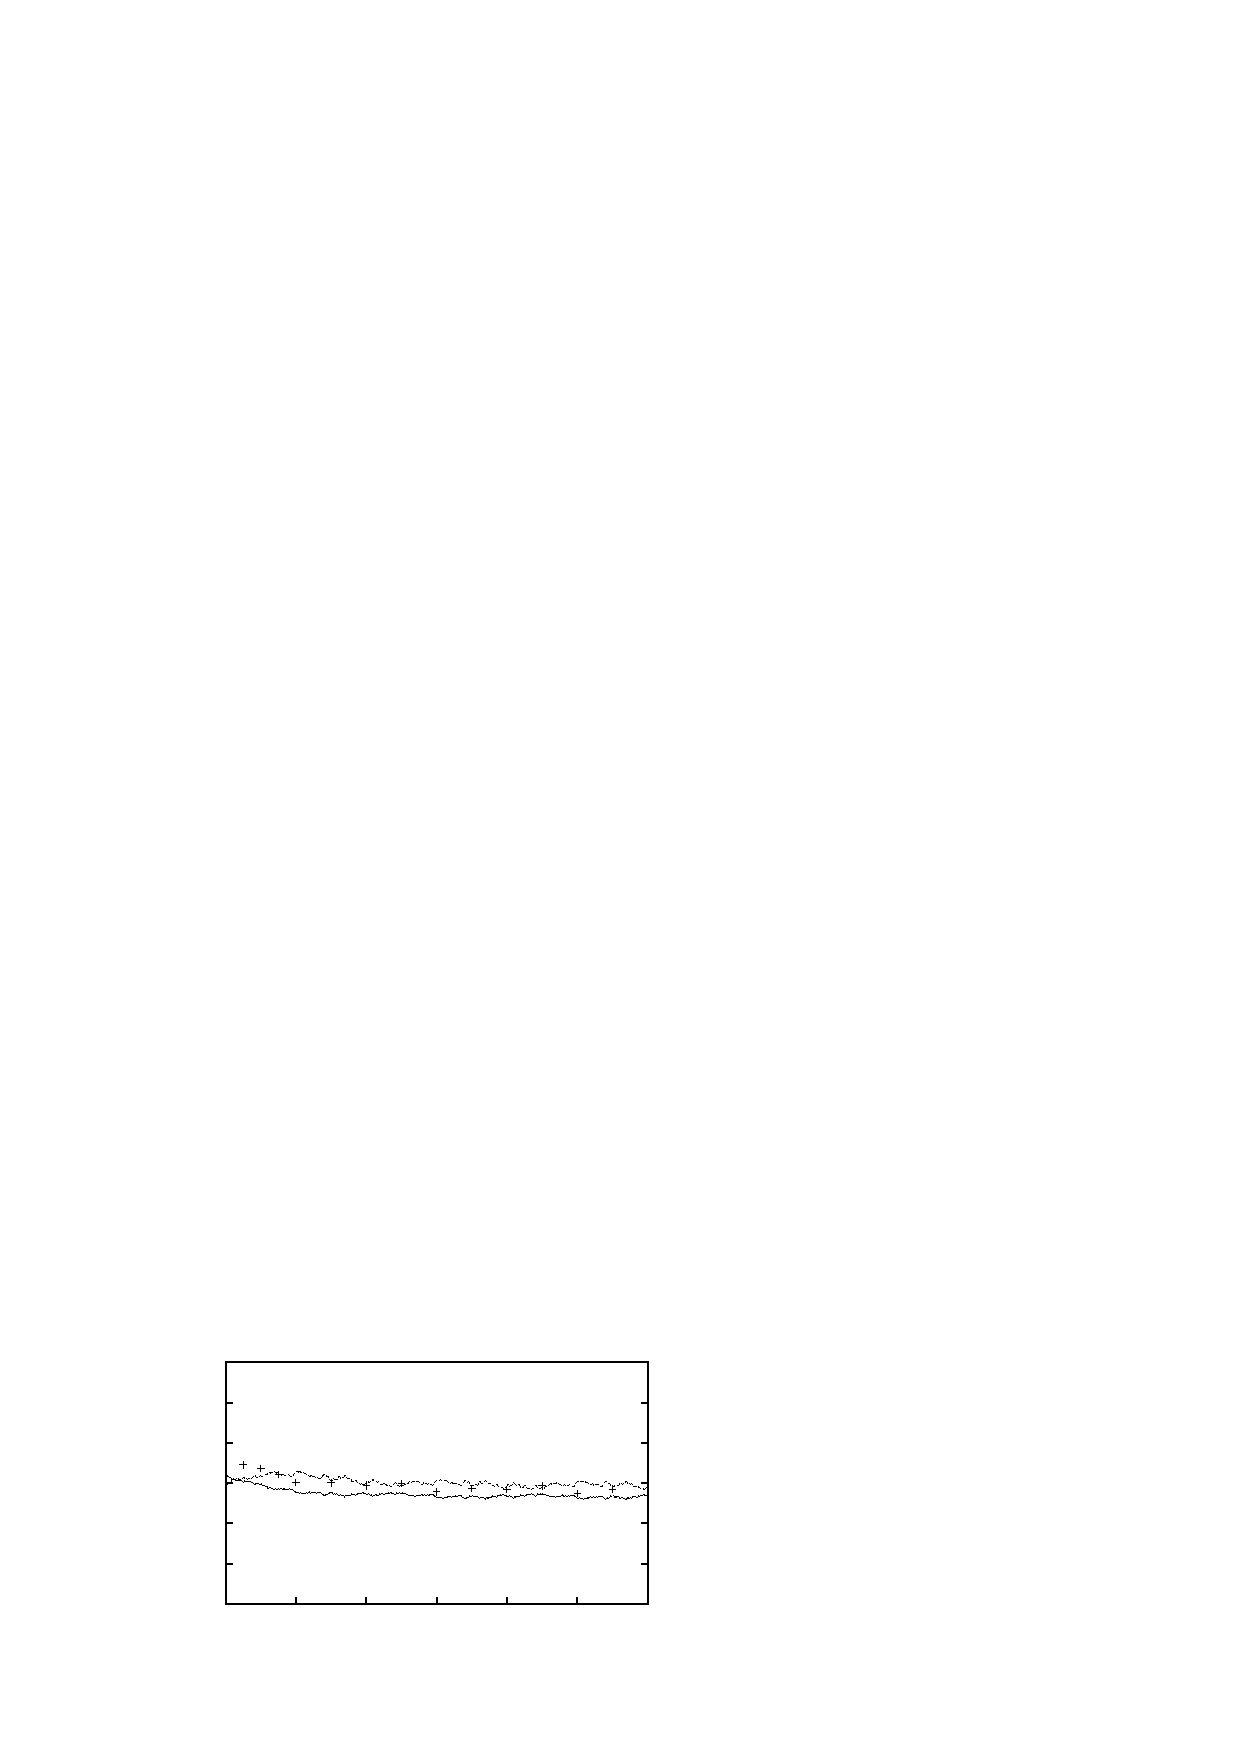
\includegraphics{realmediumJB1}}%
    \gplfronttext
  \end{picture}%
\endgroup

  \caption{Long term simulation on a sandy soil of organic matter content (left axis) and \textsc{som1} fraction (right axis) with management changing from high to medium C input. Simulated values are on the dotted line. The $\Diamond$'s indicate the initialization of \textsc{som1} for the current humus level estimated by the proposed quasi-equilibrium.}
  \label{fig:orgJB1}
\end{figure}

As can be seen, the time to reach a new equilibrium after a change in farming practice can be several centuries, which makes it safe to assume that Danish farming land is not in equilibrium. At such a time scale, not only farming practice but also climate is going to change.

\subsection{Effect of soil}
Figure~\ref{fig:JB6} and~\ref{fig:JB1} shows that the fast \textsc{som} pool (\textsc{som2}) does indeed adapt to changes in input much faster than the slow pool (\textsc{som1}), the hump in each graph is due to that effect.

\subsection{Abiotic factors}


\begin{figure}[htbp]
 % GNUPLOT: LaTeX picture with Postscript
\begingroup
  \makeatletter
  \providecommand\color[2][]{%
    \GenericError{(gnuplot) \space\space\space\@spaces}{%
      Package color not loaded in conjunction with
      terminal option `colourtext'%
    }{See the gnuplot documentation for explanation.%
    }{Either use 'blacktext' in gnuplot or load the package
      color.sty in LaTeX.}%
    \renewcommand\color[2][]{}%
  }%
  \providecommand\includegraphics[2][]{%
    \GenericError{(gnuplot) \space\space\space\@spaces}{%
      Package graphicx or graphics not loaded%
    }{See the gnuplot documentation for explanation.%
    }{The gnuplot epslatex terminal needs graphicx.sty or graphics.sty.}%
    \renewcommand\includegraphics[2][]{}%
  }%
  \providecommand\rotatebox[2]{#2}%
  \@ifundefined{ifGPcolor}{%
    \newif\ifGPcolor
    \GPcolortrue
  }{}%
  \@ifundefined{ifGPblacktext}{%
    \newif\ifGPblacktext
    \GPblacktexttrue
  }{}%
  % define a \g@addto@macro without @ in the name:
  \let\gplgaddtomacro\g@addto@macro
  % define empty templates for all commands taking text:
  \gdef\gplbacktext{}%
  \gdef\gplfronttext{}%
  \makeatother
  \ifGPblacktext
    % no textcolor at all
    \def\colorrgb#1{}%
    \def\colorgray#1{}%
  \else
    % gray or color?
    \ifGPcolor
      \def\colorrgb#1{\color[rgb]{#1}}%
      \def\colorgray#1{\color[gray]{#1}}%
      \expandafter\def\csname LTw\endcsname{\color{white}}%
      \expandafter\def\csname LTb\endcsname{\color{black}}%
      \expandafter\def\csname LTa\endcsname{\color{black}}%
      \expandafter\def\csname LT0\endcsname{\color[rgb]{1,0,0}}%
      \expandafter\def\csname LT1\endcsname{\color[rgb]{0,1,0}}%
      \expandafter\def\csname LT2\endcsname{\color[rgb]{0,0,1}}%
      \expandafter\def\csname LT3\endcsname{\color[rgb]{1,0,1}}%
      \expandafter\def\csname LT4\endcsname{\color[rgb]{0,1,1}}%
      \expandafter\def\csname LT5\endcsname{\color[rgb]{1,1,0}}%
      \expandafter\def\csname LT6\endcsname{\color[rgb]{0,0,0}}%
      \expandafter\def\csname LT7\endcsname{\color[rgb]{1,0.3,0}}%
      \expandafter\def\csname LT8\endcsname{\color[rgb]{0.5,0.5,0.5}}%
    \else
      % gray
      \def\colorrgb#1{\color{black}}%
      \def\colorgray#1{\color[gray]{#1}}%
      \expandafter\def\csname LTw\endcsname{\color{white}}%
      \expandafter\def\csname LTb\endcsname{\color{black}}%
      \expandafter\def\csname LTa\endcsname{\color{black}}%
      \expandafter\def\csname LT0\endcsname{\color{black}}%
      \expandafter\def\csname LT1\endcsname{\color{black}}%
      \expandafter\def\csname LT2\endcsname{\color{black}}%
      \expandafter\def\csname LT3\endcsname{\color{black}}%
      \expandafter\def\csname LT4\endcsname{\color{black}}%
      \expandafter\def\csname LT5\endcsname{\color{black}}%
      \expandafter\def\csname LT6\endcsname{\color{black}}%
      \expandafter\def\csname LT7\endcsname{\color{black}}%
      \expandafter\def\csname LT8\endcsname{\color{black}}%
    \fi
  \fi
  \setlength{\unitlength}{0.0500bp}%
  \begin{picture}(5760.00,3024.00)%
    \gplgaddtomacro\gplbacktext{%
      \csname LTb\endcsname%
      \put(1034,1144){\makebox(0,0)[r]{\strut{} 0}}%
      \put(1034,1359){\makebox(0,0)[r]{\strut{} 0.2}}%
      \put(1034,1575){\makebox(0,0)[r]{\strut{} 0.4}}%
      \put(1034,1790){\makebox(0,0)[r]{\strut{} 0.6}}%
      \put(1034,2006){\makebox(0,0)[r]{\strut{} 0.8}}%
      \put(1034,2221){\makebox(0,0)[r]{\strut{} 1}}%
      \put(1034,2437){\makebox(0,0)[r]{\strut{} 1.2}}%
      \put(1034,2652){\makebox(0,0)[r]{\strut{} 1.4}}%
      \put(1166,924){\makebox(0,0){\strut{}01}}%
      \put(1542,924){\makebox(0,0){\strut{}02}}%
      \put(1894,924){\makebox(0,0){\strut{}03}}%
      \put(2257,924){\makebox(0,0){\strut{}04}}%
      \put(2622,924){\makebox(0,0){\strut{}05}}%
      \put(2985,924){\makebox(0,0){\strut{}06}}%
      \put(3349,924){\makebox(0,0){\strut{}07}}%
      \put(3713,924){\makebox(0,0){\strut{}08}}%
      \put(4089,924){\makebox(0,0){\strut{}09}}%
      \put(4453,924){\makebox(0,0){\strut{}10}}%
      \put(4817,924){\makebox(0,0){\strut{}11}}%
      \put(5181,924){\makebox(0,0){\strut{}12}}%
      \put(484,1952){\rotatebox{90}{\makebox(0,0){\strut{}}}}%
      \put(3342,594){\makebox(0,0){\strut{}Month}}%
    }%
    \gplgaddtomacro\gplfronttext{%
      \csname LTb\endcsname%
      \put(2487,173){\makebox(0,0)[r]{\strut{}JB1}}%
      \csname LTb\endcsname%
      \put(3738,173){\makebox(0,0)[r]{\strut{}JB6}}%
    }%
    \gplbacktext
    \put(0,0){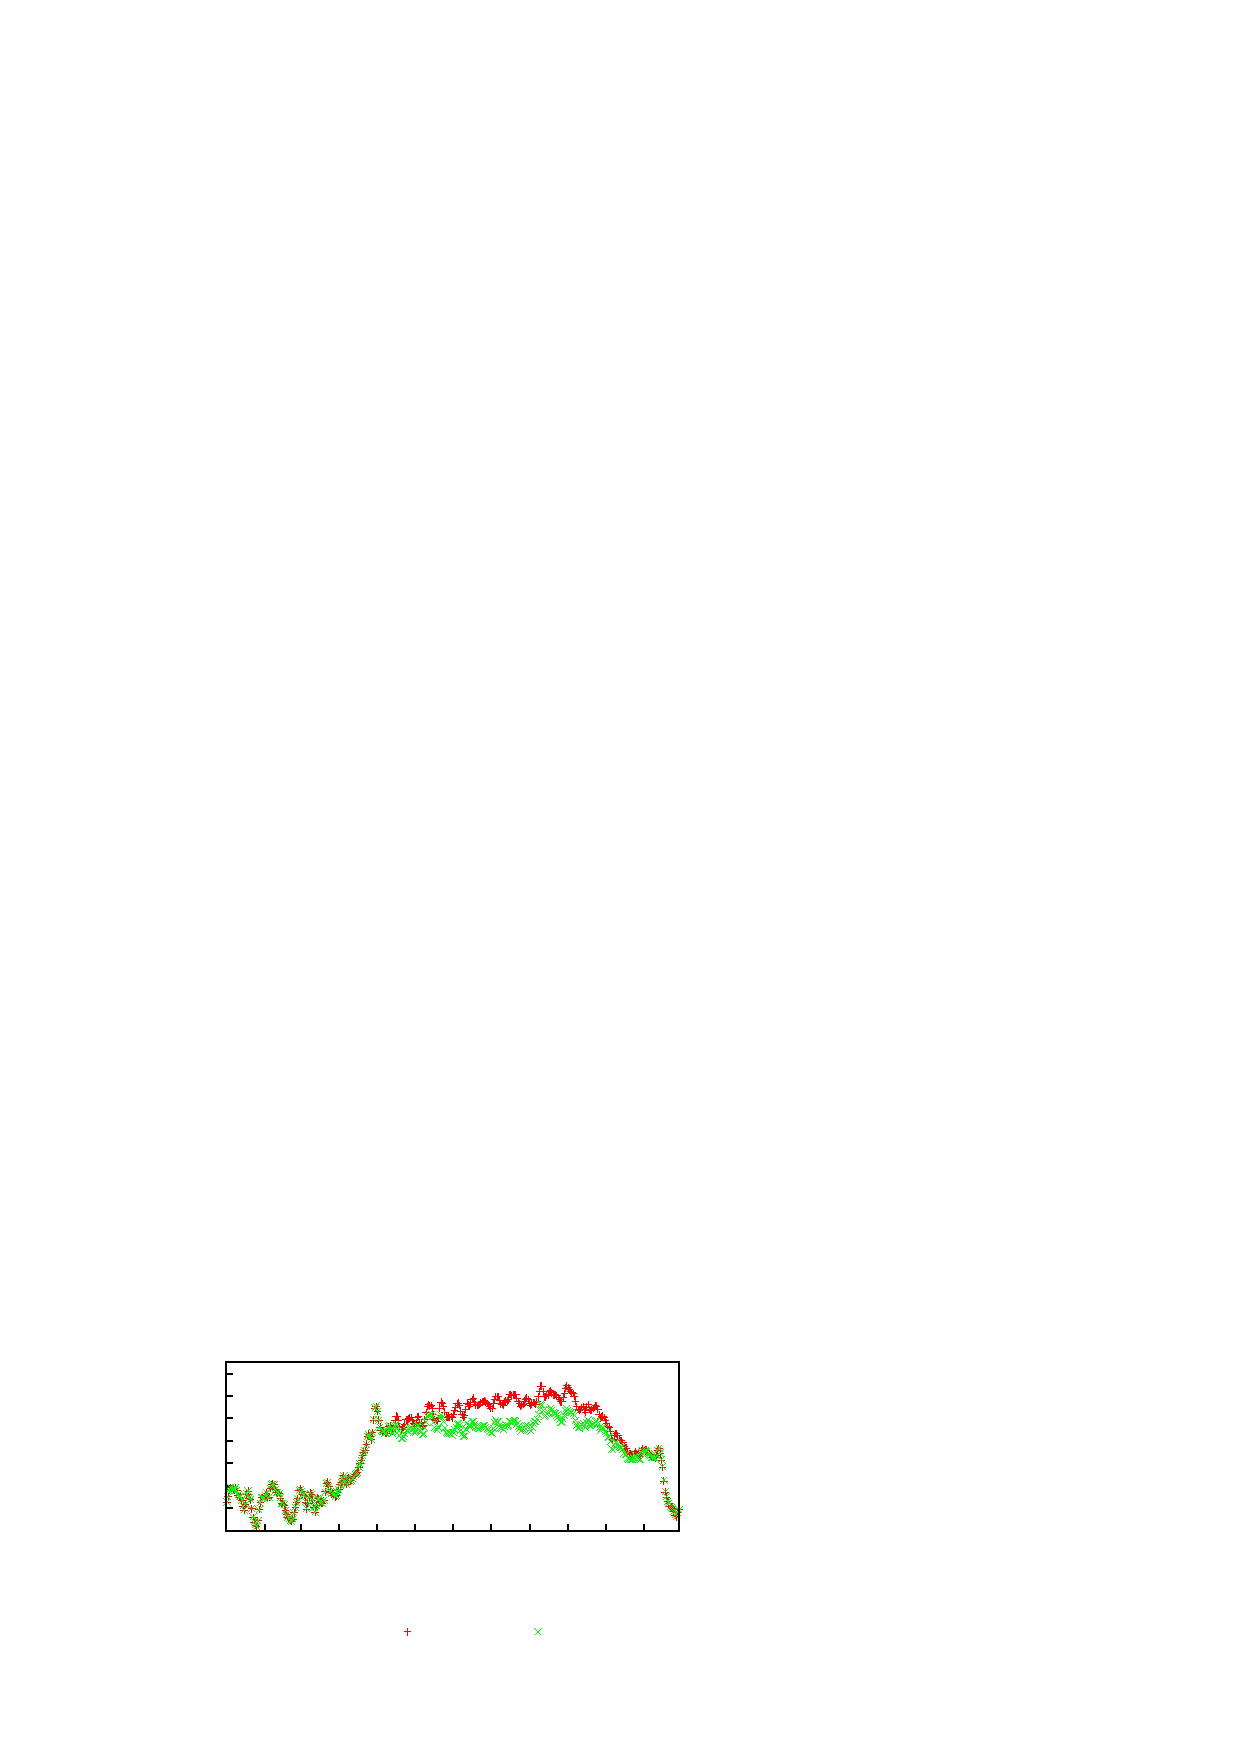
\includegraphics{abioticYear}}%
    \gplfronttext
  \end{picture}%
\endgroup

  \caption{Yearly variation of abiotic factor for sandy and sandy loam soil. The $\Diamond$'s ....}
  \label{fig:year}
\end{figure}

\begin{figure}[htbp]
 %GNUPLOT: LaTeX picture with Postscript
\begin{picture}(0,0)%
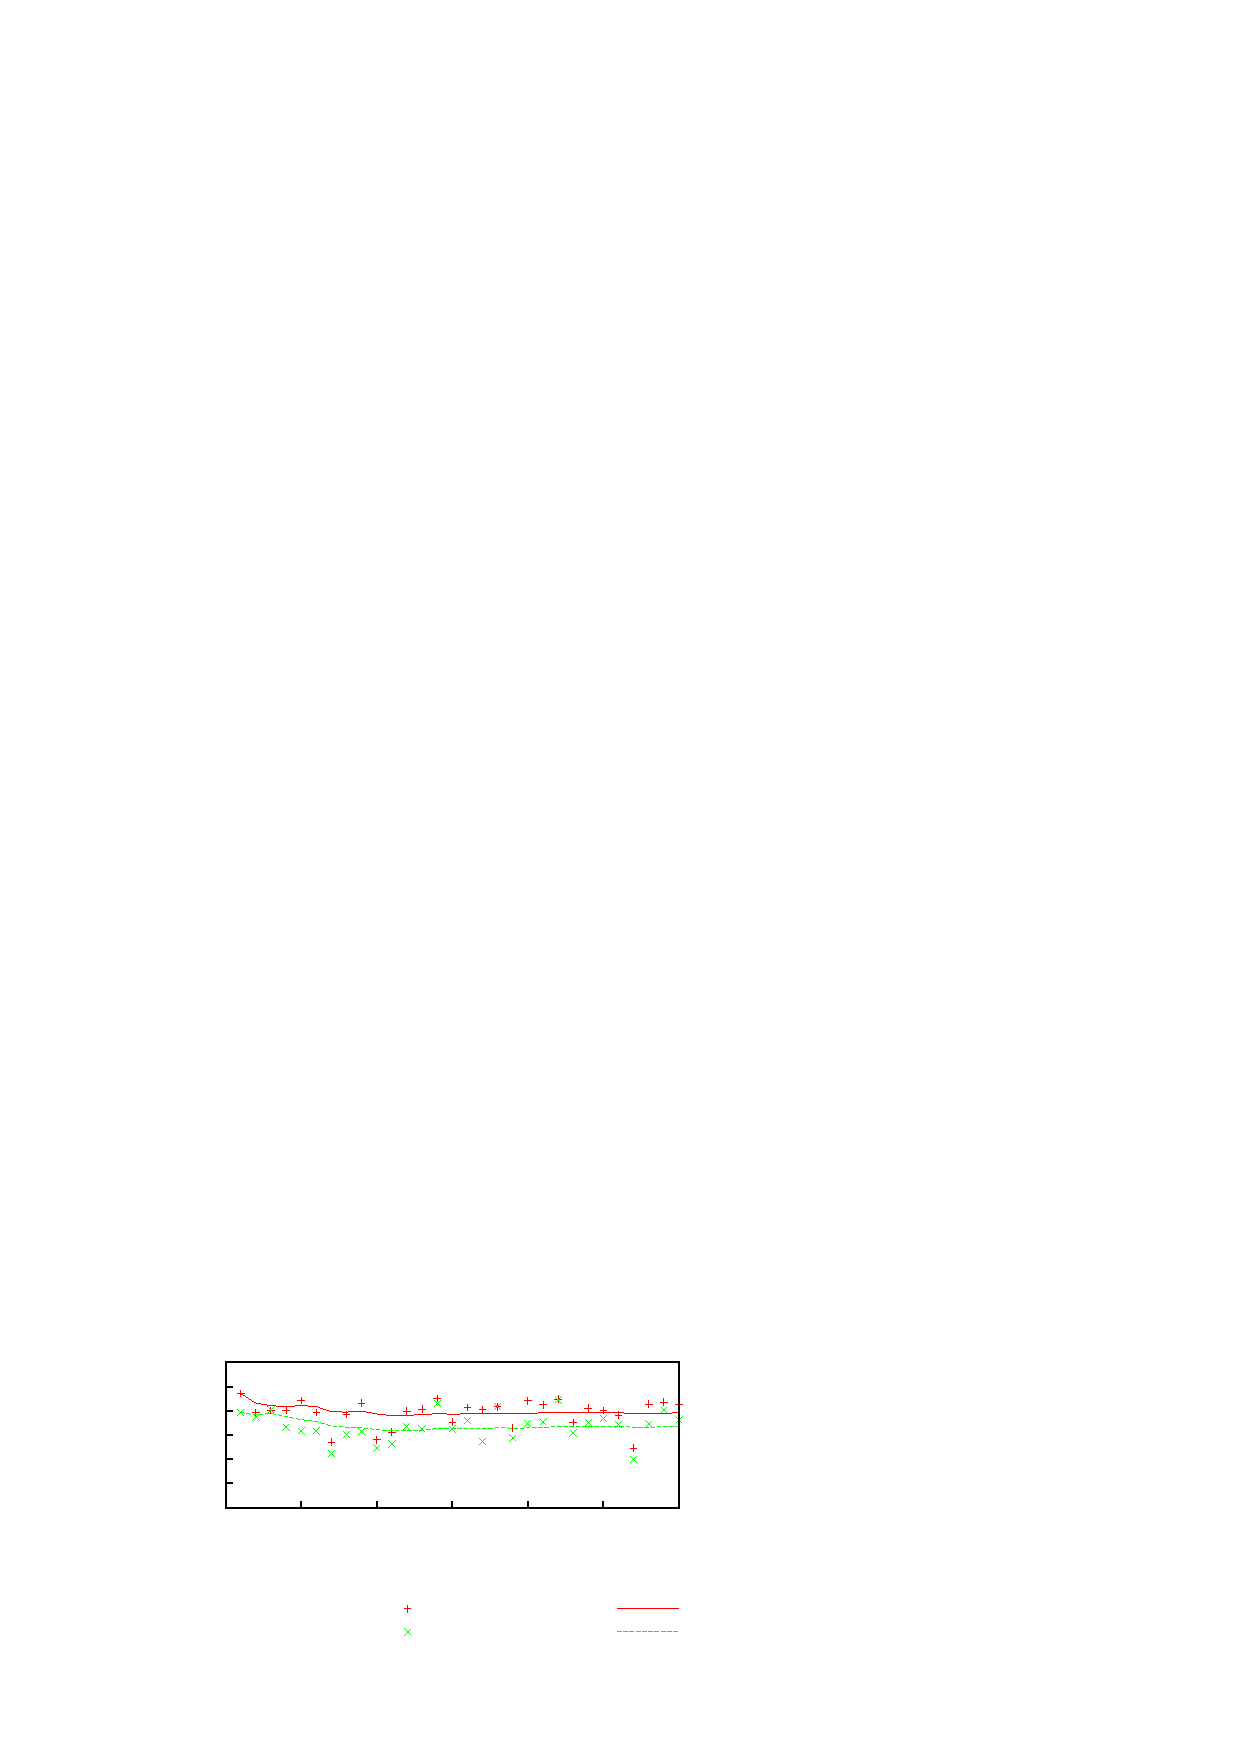
\includegraphics{abiotic30}%
\end{picture}%
\begingroup
\setlength{\unitlength}{0.0200bp}%
\begin{picture}(18000,10800)(0,0)%
\put(2200,3300){\makebox(0,0)[r]{\strut{} 0.3}}%
\put(2200,4458){\makebox(0,0)[r]{\strut{} 0.4}}%
\put(2200,5617){\makebox(0,0)[r]{\strut{} 0.5}}%
\put(2200,6775){\makebox(0,0)[r]{\strut{} 0.6}}%
\put(2200,7933){\makebox(0,0)[r]{\strut{} 0.7}}%
\put(2200,9092){\makebox(0,0)[r]{\strut{} 0.8}}%
\put(2200,10250){\makebox(0,0)[r]{\strut{} 0.9}}%
\put(2475,2750){\makebox(0,0){\strut{}2000}}%
\put(4926,2750){\makebox(0,0){\strut{}2005}}%
\put(7376,2750){\makebox(0,0){\strut{}2010}}%
\put(9826,2750){\makebox(0,0){\strut{}2015}}%
\put(12276,2750){\makebox(0,0){\strut{}2020}}%
\put(14726,2750){\makebox(0,0){\strut{}2025}}%
\put(17175,2750){\makebox(0,0){\strut{}2030}}%
\put(550,6775){\rotatebox{90}{\makebox(0,0){\strut{}Abiotic factor}}}%
\put(9825,1925){\makebox(0,0){\strut{}Year}}%
\put(5200,825){\makebox(0,0)[l]{\strut{}JB1}}%
\put(5200,275){\makebox(0,0)[l]{\strut{}JB6}}%
\put(13650,825){\makebox(0,0)[l]{\strut{}JB1-average}}%
\put(13650,275){\makebox(0,0)[l]{\strut{}JB6-average}}%
\end{picture}%
\endgroup
\endinput

  \caption{Yearly variation of abiotic factor for sandy and sandy loam soil. The $\Diamond$'s ....}
  \label{fig:30}
\end{figure}


\subsection{Limitations}

When using the current input levels, the quasi-equilibrium assumption will give very poor, even physically impossible estimates right after a large change in input level. This is because the \textsc{som2} pool will not yet have had any chance to adopt to the new input level. With the current model, the \textsc{som2} pool needs several decades to catch up with changes in input. This means that the quasi-equilibrium assumption is still suspect in a modern agricultural country like Denmark.

A model specific bound on the relative size of \textsc{som1} has been introduced. Our long term simulations has shown that the \textsc{som1} fraction stay within the interval 30\% --- 70\%. If the quasi-equilibrium give a value outside that interval, the \textsc{som1} fraction will be set to that nearest boundary, and the initialization will be redone. More precisely, if the quasi-equilibrium gives a \textsc{som1} higher than 70\%, equation~\ref{eq:dsom2} will be replaced with the new equation:

\begin{displaymath}
    \mbox{\textsc{som1}} = 70\%\> (\mbox{\textsc{som1}} + \mbox{\textsc{som2}})
\end{displaymath}
and similar for a \textsc{som1} below 30\%.

While the humus content in especially figure~\ref{fig:JB1} fluctuates with rotation, season and climate, the simulated \textsc{som1} fraction stay relatively stable. This is because most of the minor fluctuations happens in the \textsc{aom} and \textsc{smb} pools, the slower \textsc{som2} does not have time to adapt. This also explains the relatively noise on the initialization points, the quasi-equilibrium assumption over-adapts to such short terms changes.

\subsection{Usability}

This initialization procedure is particular strong with regard to changes in number of pools. Adding a new pool (for instance $\Delta\mbox{\textsc{smb}}i$) will add one more equation and two new unknown parameters ($a$ and $b$ for the ${\textsc{smb}}i$ pool ???? ER DET RIGTIGT??). The generalized form for $\Delta\mbox{\textsc{smb}}i$ and $\Delta\mbox{\textsc{som}}j$ is:

\begin{equation}
   \begin{array}{rclcr}
      \label{eq:dsmb}
      \Delta\mbox{\textsc{smb}}i &=& \displaystyle
      \sum_{k=1}^{\mbox{\tiny\#\textsc{smb}}} a_{i,k}\,\mbox{\textsc{smb}}k +
      \sum_{l=1}^{\mbox{\tiny\#\textsc{som}}} b_{i,l}\,\mbox{\textsc{som}}l +
      c_i \Delta\mbox{\textsc{aom}}
      &;&i = 1\ldots\mbox{\#\textsc{smb}}
    \end{array}
  \end{equation}
\begin{equation}
   \begin{array}{rclcr}
      \Delta\mbox{\textsc{som}}j &=& \displaystyle
      \sum_{k=1}^{\mbox{\tiny\#\textsc{smb}}} d_{j,k}\,\mbox{\textsc{smb}}k +
      \sum_{l=1}^{\mbox{\tiny\#\textsc{som}}} e_{j,l}\,\mbox{\textsc{som}}l +
      f_j \Delta\mbox{\textsc{aom}}
      &;&j = 1\ldots\mbox{\#\textsc{som}}
    \end{array}
  \end{equation}

\section{Conclusion}

The initialization method developed here is easy to understand and to do by the user. The two mandatory numbers are the total content of organic matter, and an estimate of how much carbon has been added to the system per year in the recent decades. The total content of organic matter is directly measurable and the carbon input estimated by the user, for example from the use of \daisy{} simulations. None of the these numbers need to be changed when the model itself is changed.

Abiotiske faktorer kan vi godt give som statiske faktorer ligeledes med C-input (variationen indenfor et s�dskifte). Vi kan ikke hvis s�dskifte varierer.

De �rlige fluktioner i vejret kan vi godt ignorerer og stadig f� et rimeligt godt bud med den dynamiske model - men ikke en systematisk variation over �rene (global change).


\addcontentsline{toc}{section}{\numberline{}References}
\bibliography{../daisy}

\end{document}

Daisy - sm� tidsskridt, kort tidshorisont (h�st og N-udvaskning) CO2 fluxe. Vejr (drivende variable) meget dynamisk indefor �ret og mellem �r.
Hypotese: at vi kan initialiserer fordelingen af C mellem SOM puljer i en meget dynamisk model med en statisk model.


%%% Local Variables:
%%% mode: latex
%%% TeX-master: t
%%% End:
